\chapter[METHODS AND METHODOLOGY]{\huge METHODS AND METHODOLOGY}

\begin{figure}[h!]
	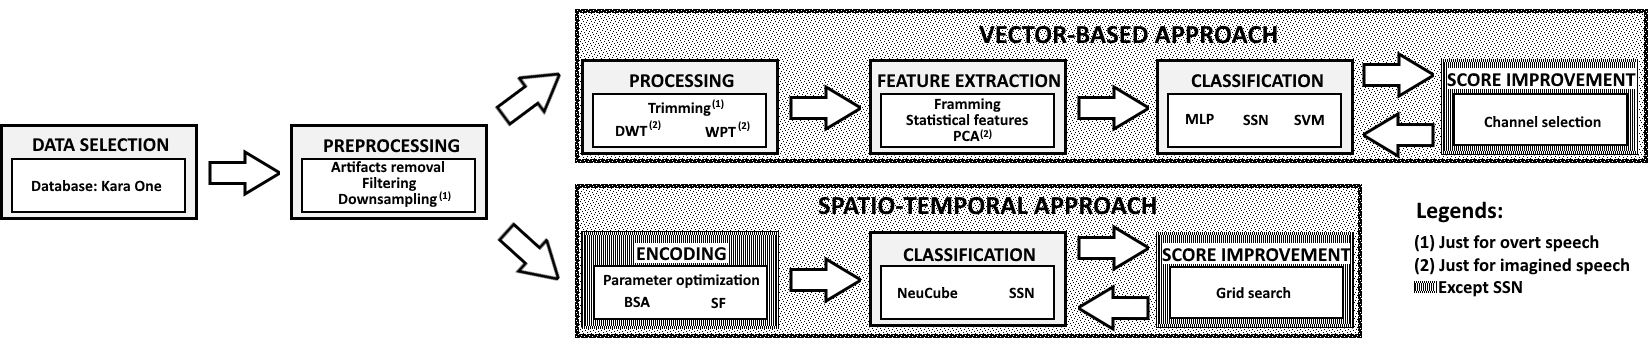
\includegraphics[width=\linewidth]{Figures/Diagram.png}
	\centering
	\caption{General block diagram of the methodology followed.}
	\label{Fig: Diagram}
\end{figure}

In this chapter is described the methodology followed in this work to classify imagined and overt speech samples. Figure \ref{Fig: Diagram} shows the block diagram with each step involved in the classification. The steps for both classifier approaches, Vector-Based and Spatio-Temporal, are differentiated with their particular methods. Besides, the methods required for the preprocessing and processing of imagined and overt speech signals are distinguished. The following sections detail the work done in each step.

\section{Data Selection}
The samples used in this work were obtained from the database Kara One \cite{karaone}, which contains EEG recordings captured with a 64-channel Neuroscan Quick cap, using the 10-20 system and sampled at 1 Kilohertz. These recordings were taken from 14 subjects and stored in individual EEGLab set files.\\

In addition, each set file contains, most of the cases, samples of 12 trials from 7 phonemic/syllabic classes (/iy/, /uw/, /piy/, /tiy/, /diy/, /m/, /n/ ) and 4 word classes (pat, pot, knew, gnaw), each. According to \cite{zhao2015classifying}, for each class recording, the subjects were instructed to relax by 5 seconds, followed by 2 seconds of stimuli in where the participant prepare his/her articulators. Then, the participant was told to imagine speaking the phoneme or word continuously by 5 seconds, followed by a variable interval to pronounce the same class.\\

\begin{figure}[h!]
	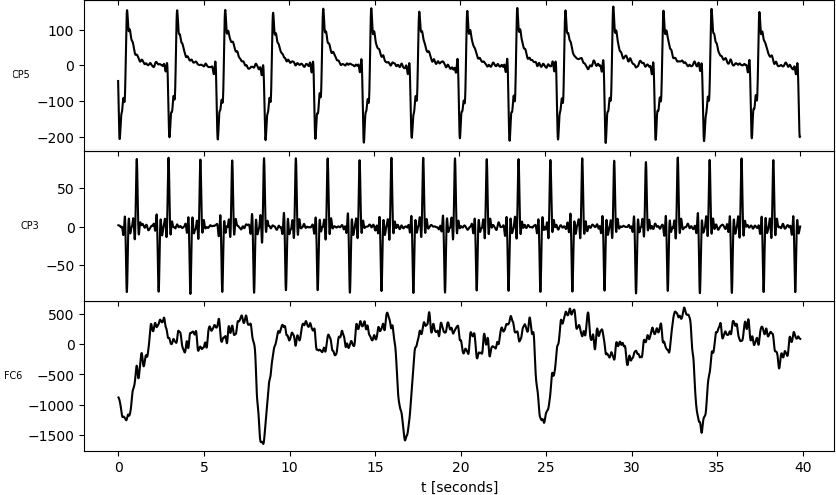
\includegraphics[scale=0.4]{Figures/Rejected_Signals.png}
	\centering
	\caption{Some examples of signals from rejected samples.}
	\label{Fig: Rejected}
\end{figure}

\begin{table}[h!]
\caption{Samples used for class and user.}
\centering
\begin{tabular}{|c|c|c|c|c|c|}\hline
	\textbf{Class$\backslash$Subject}&\textbf{$S_{1}$}&\textbf{$S_{2}$}&\textbf{$S_{3}$}&\textbf{$S_{4}$}&\textbf{$S_{5}$}\\\hline
	\textbf{\textit{/diy/}}&15&8&11&9&0\\\hline
	\textbf{\textit{gnaw}}&15&5&12&8&11\\\hline
	\textbf{\textit{/iy/}}&15&8&12&11&6\\\hline
	\textbf{\textit{/knew/}}&15&10&12&8&12\\\hline
	\textbf{\textit{/m/}}&15&6&12&8&7\\\hline
	\textbf{\textit{/n/}}&14&7&12&8&6\\\hline
	\textbf{\textit{pat}}&15&6&12&9&12\\\hline
	\textbf{\textit{/piy/}}&15&6&11&7&9\\\hline
	\textbf{\textit{pot}}&15&7&12&8&11\\\hline
	\textbf{\textit{/tiy/}}&15&7&12&8&6\\\hline
	\textbf{\textit{/uw/}}&15&5&11&3&8\\\hline
	\textbf{TOTAL}&\textbf{164}&\textbf{75}&\textbf{129}&\textbf{87}&\textbf{88}\\\hline
\end{tabular}
\label{Table: Subj_Class}
\end{table}

For this work, the corresponding 5 seconds imagined speech, as well as the following overt speech samples, were selected from the database. However, some of the \linebreak[4]preprocessed signals were discarded after observing notorious periodicities in time not seen in other revised related works. Figure \ref{Fig: Rejected} shows some examples of signals presenting this problem.\\

The decision over signals with that problem was out of the scope for this work. Due to that, for this work were used just some samples from the subjects \textit{MM05}, \textit{MM08}, \textit{MM10}, \textit{MM18} and \textit{MM19} (named here as $S_{1}$, $S_{2}$, $S_{3}$, $S_{4}$ and $S_{5}$, respectively), that in total gave 543 samples per mental activity. Table \ref{Table: Subj_Class} shows the number of samples selected by subject and class.\\

Also, it was followed the same binary grouping as in \cite{zhao2013combining,zhao2015classifying}. That is, the original 11 classes were grouped into two new classes, building different binary sets based on their phonological relation. These binary sets were: vowel-only vs. consonant (C/V), presence of nasal ($\pm$Nasal), presence of bilabial ($\pm$Bilabial), presence of high-front vowel ($\pm$/iy/), and presence of high-back vowel ($\pm$/uw/).\\

While in \cite{zhao2013combining,zhao2015classifying} reported results from the most unbalanced pair of sets ($\pm$/uw/ and C/V), in order to avoid biased results, for the experiments reported here were used the less two unbalanced binary sets: $\pm$Nasal or $\pm$Bilabial, both with 340 samples in one class and 203 in the other. In Table \ref{Table: Binary_Class} are shown the samples' distribution on each phonological pair of sets, as well as the association of the original 11 classes with the new binary classes (class 1 or 2).

\begin{table}[h!]
	\centering
	\caption{Binary grouping and samples per binary class.}
	\begin{tabular}{|*{7}{c|}}
		\cline{3-7}
		\multicolumn{2}{c|}{\multirow{2}{*}{}}&\multicolumn{5}{c|}{		\textbf{BINARY CLASSES}}\\\cline{3-7}
		\multicolumn{2}{c|}{}&\textbf{V/C}&\textbf{$\pm$Nasal}&\textbf{$\pm$Bilabial}&\textbf{$\pm$iy}&\textbf{$\pm$uw}\\\hline
		\multirow{11}{*}{\begin{sideways}\textbf{ORIGINAL CLASSES}\end{sideways}}&\textbf{/diy/}&2&1&1&2&1\\\cline{2-7}
		&\textbf{gnaw}&2&2&1&1&1\\\cline{2-7}
		&\textbf{/iy/}&1&1&1&2&1\\\cline{2-7}
		&\textbf{knew}&2&2&1&1&1\\\cline{2-7}
		&\textbf{/m/}&2&2&2&1&1\\\cline{2-7}
		&\textbf{/n/}&2&2&1&1&1\\\cline{2-7}
		&\textbf{pat}&2&1&2&1&1\\\cline{2-7}
		&\textbf{/piy/}&2&1&2&2&1\\\cline{2-7}
		&\textbf{pot}&2&1&2&1&1\\\cline{2-7}
		&\textbf{/tiy/}&2&1&1&2&1\\\cline{2-7}
		&\textbf{/uw/}&1&1&1&2&2\\\hline
		\multicolumn{2}{|c|}{\textbf{SAMPLES}}&\textbf{94$\mid$449}&\textbf{340$\mid$203}&\textbf{340$\mid$203}&\textbf{352$\mid$191}&\textbf{501$\mid$42}\\\hline
	\end{tabular}%
	\label{Table: Binary_Class}
\end{table}%

\section{Preprocessing}

\begin{figure}[h!]
	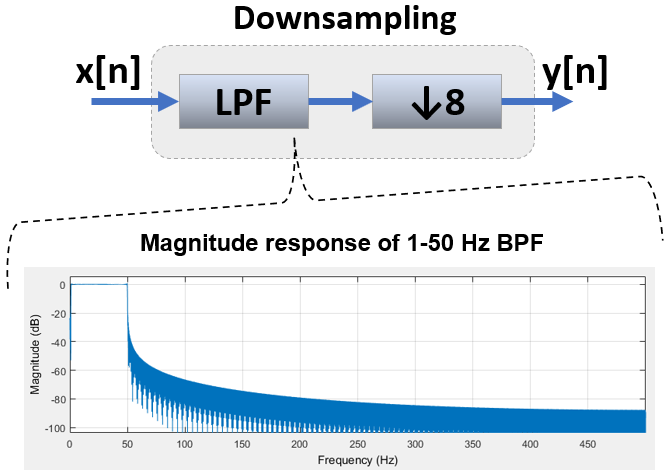
\includegraphics[scale=0.4]{Figures/Downsampling.png}
	\centering
	\caption{Downsampling process applied to all signals.}
	\label{Fig: Downsampling}
\end{figure}
For this work were used the preprocessed signals from the database Kara One. Therefore, this step was the same as in \cite{zhao2015classifying,zhao2013combining}, which consisted of the following steps:
\begin{enumerate}
	\item Removal of ocular artifacts using blind source separation with EEGLAB \cite{delorme2004eeglab}.
	\item Band-pass filtering (BPF) from 1 to 50 Hz.
	\item Mean values subtraction from each channel.
	\item Small Laplacian filtering, using the neighborhood of adjacent channels.
\end{enumerate}

Additionally, in the case of imagined speech, signals were downsampled by a factor of 8, resulting in 125 samples per second (originally were 1000). This step was necessary for these data due to the spectral analysis done with wavelets in the next step. Figure \ref{Fig: Downsampling} exemplify this process. When a signal is downsampled, it is required to be beforehand filtered with an LPF to avoid aliasing.\\

However, as mentioned above, instead, all data were previously filtered by a BPF, which worked for this purpose. Also, the idea of downsampling was to reduce data points and reject useless frequency bands to work with the wavelets just over the bandpass 0-62.5 Hz.
\section[Processing, Feature Extraction and Classification Approaches]{\texorpdfstring{Processing, Feature Extraction and\\ Classification Approaches}{Processing, Feature Extraction and Classification Approaches}}
In this section are described the processing, feature extraction, and classification steps for both approaches used in this work: Vector-Based and Spatio-Temporal. It is also described the processes for the classifier that can combine both approaches.

\subsection{Vector-Based}
\subsubsection{Processing}
For overt speech samples, this step consisted of identifying from all the time points just those that correspond when the subjects pronounced the classes. That is, to extract information just from the intervals of actual overt speech. These intervals were identified with the endpoints detection algorithm for isolated utterances proposed in \cite{rabiner1975algorithm} and broadly used in speech recognition research.  Indeed, just the energy from the acoustic signals (also available in the database) was computed.\\

\begin{figure}[h!]
	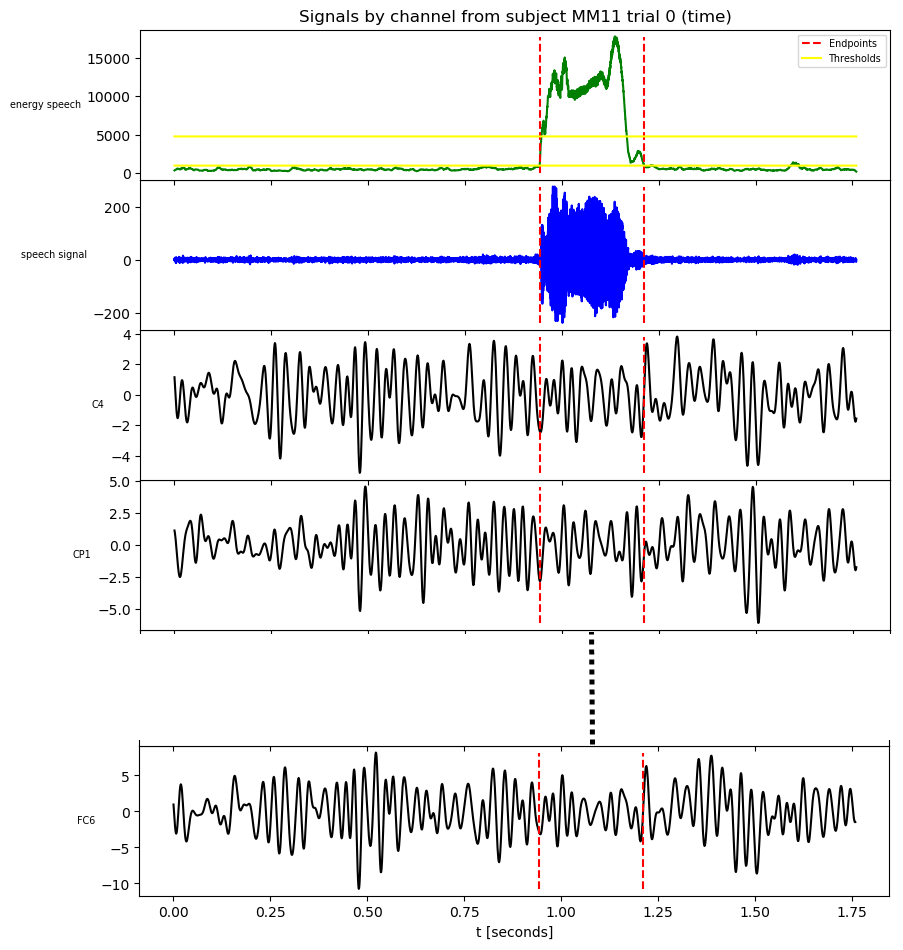
\includegraphics[scale=0.4]{Figures/Overt_speech_trim.png}
	\centering
	\caption{Automatic overt speech trimming based on acoustic endpoints.}
	\label{Fig: Trimming}
\end{figure}

\begin{figure}[h!]
\centering
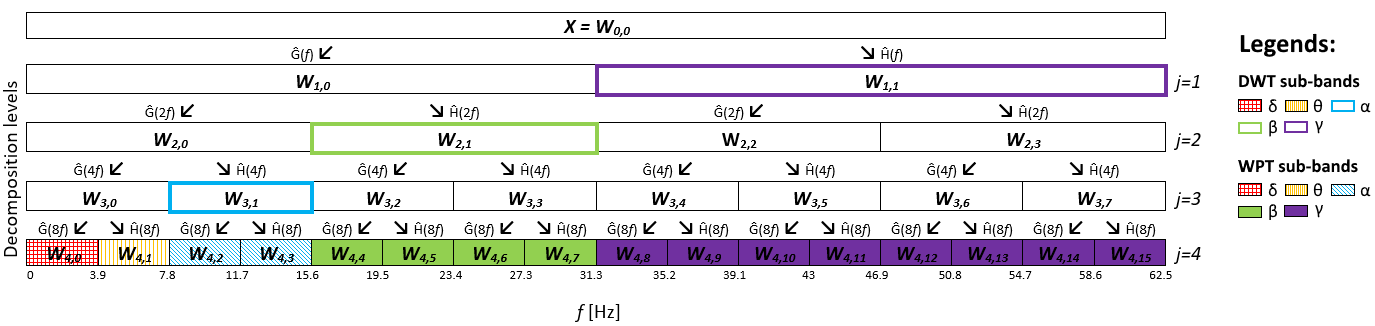
\includegraphics[width=\linewidth]{Figures/Wavelets.png}
\caption{Wavelet decomposition tree with 4 levels.}
\label{Fig: Wavelet_decomp}
\end{figure}

Figure \ref{Fig: Trimming} shows, from the top to the bottom, the computed energy, the acoustic signal, and some EEG signals from the same sample. In the case of the energy plot, the horizontal yellow lines represent the thresholds computed in the algorithm to state the endpoints. Therefore, the vertical red dashed lines across all the plots represent the start and end of the resulting interval that was used to trim the signals.\\

In some cases, the algorithm failed due to noise with high energy added to the acoustic signals. That is, sometimes, the starting point or ending point was not found. For such cases, a program was implemented to select the endpoints manually by taking as reference the recordings and some plots like those from Figure \ref{Fig: Trimming}.\\

Also, a downsampling step (neither a wavelet processing) was not performed for overt speech signals. This step was not done because the signals (after been trimmed) had few sample points that were considered just enough to compute features.\\

On the other hand, for imagined speech samples was necessary to process all the time points (equivalent to 5 seconds) since there were no external references to identify the exact moment when the people thought about the classes. It is just known that they were instructed to think about the classes continuously during that time interval.\\

The processing step consisted of computing the wavelet coefficients from the signals with two different approaches: DWT and WPT. A db4 function was used as a mother wavelet, and the coefficients were computed with the MODWPT \ref{walden1998phase} function of MATLAB, which has the advantage of making alignment in time with the original signal. Also, MODWPT avoids downsampling, which means that all resulting wavelet coefficient sets have the same length.\\

Figure \ref{Fig: Wavelet_decomp} represents the 4 levels of decomposition applied over the imagined speech signals with DWT and WPT.  \small\textbf{\textit{X}} represents the coefficients after correlating the EEG signal with the mother wavelet. $\hat{G}(\lambda f) $ represents the LPF and $\hat{H}(\lambda f)$ the HPF applied on the $j$  decomposition level (where $\lambda=2^{j}$). The interval of the resulting sub-bands is shown at the bottom of the figure (in Hz). Notice that the Nyquist frequency is 62.5 Hz due to the previous downsampling step.\\

For both approaches, the coefficient sets \textbf{\textit{W$_{4,0}$}} and \textbf{\textit{W$_{4,1}$}} correspond closely to the $\delta$ and $\theta$ subbands, respectively. In the case of using DWT, the coefficients \textbf{\textit{W$_{3,1}$}}, \textbf{\textit{W$_{2,1}$}}, and \textbf{\textit{W$_{1,1}$}} correspond to the $\alpha$, $\beta$ and $\gamma$ sub-bands, respectively, resulting 5 signals to analyze. Whereas using WPT, the coefficients \textbf{\textit{W$_{4,2}$}} and \textbf{\textit{W$_{4,3}$}} correspond to the $\alpha$ sub-band, the coefficient sets from \textbf{\textit{W$_{4,4}$}} to \textbf{\textit{W$_{4,7}$}} correspond to the $\beta$ sub-band, and the coefficient sets from \textbf{\textit{W$_{4,8}$}} to \textbf{\textit{W$_{4,15}$}} correspond to the $\gamma$ sub-band, resulting 16 signals to analyze.\\

\begin{figure}[h!]
	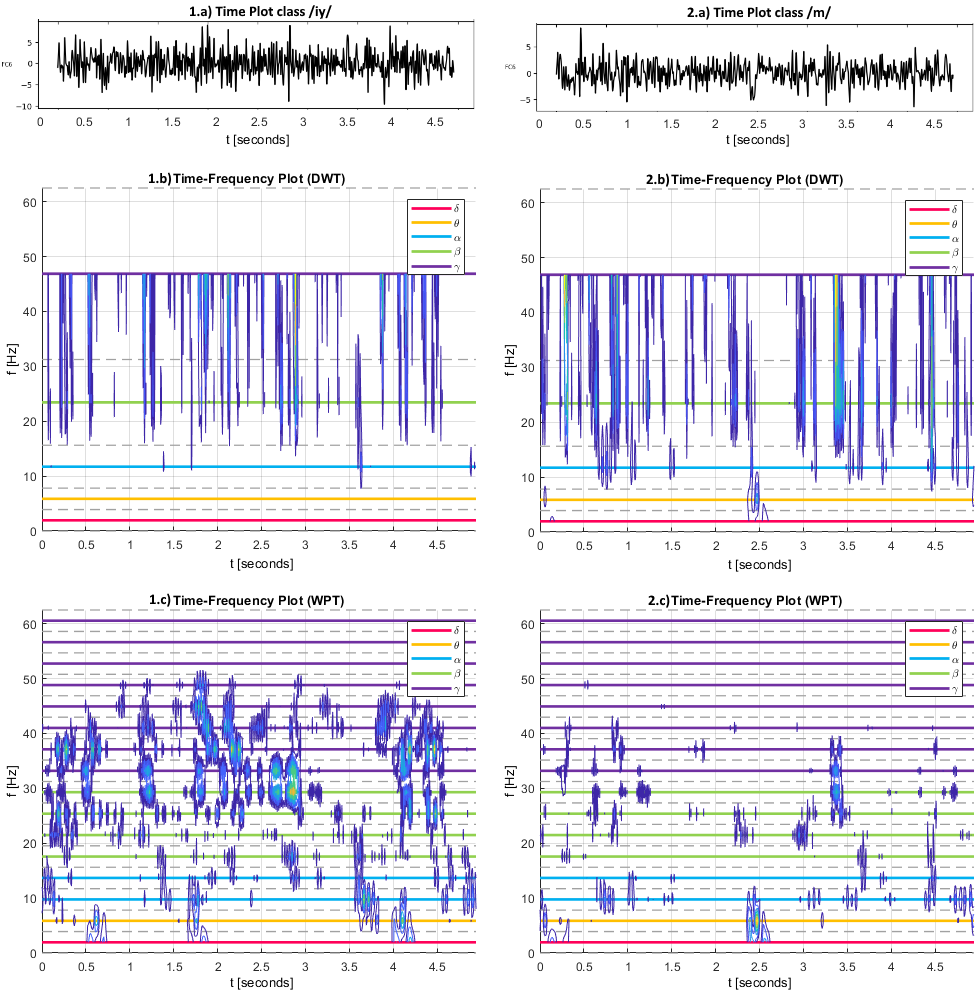
\includegraphics[width=\linewidth]{Figures/Time_Freq_Wavelet.png}
	\centering
	\caption{Examples of Wavelet energy analysis by sub-band.}
	\label{Fig: Wavelet_freq_time}
\end{figure}

Besides, Figure \ref{Fig: Wavelet_freq_time} shows examples of wavelet decomposition over FC6 channel signals from the same subject when imagined the class \textit{/iy/} (left column of plots) and \textit{/m/} (right column of plots). Plots 1.a) and 2.a) represent the signals in continuous time (seconds), while plots 1.b)-2.b) and 1.c)-2.c) show the time-frequency energy locations after applying DWT and WPT, repectively, over the signals with the MODWPT function.\\

Such time-frequency plots show the central frequencies of each filter used in the wavelet decompositions. These central frequencies are represented with horizontal lines, that are distinguished by colors associated with $\delta$, $\theta$, $\alpha$, $\beta$ and $\gamma$ sub-bands. Also, the dashed gray lines represent the borderlines between filters.\\

\begin{figure}[h!]
	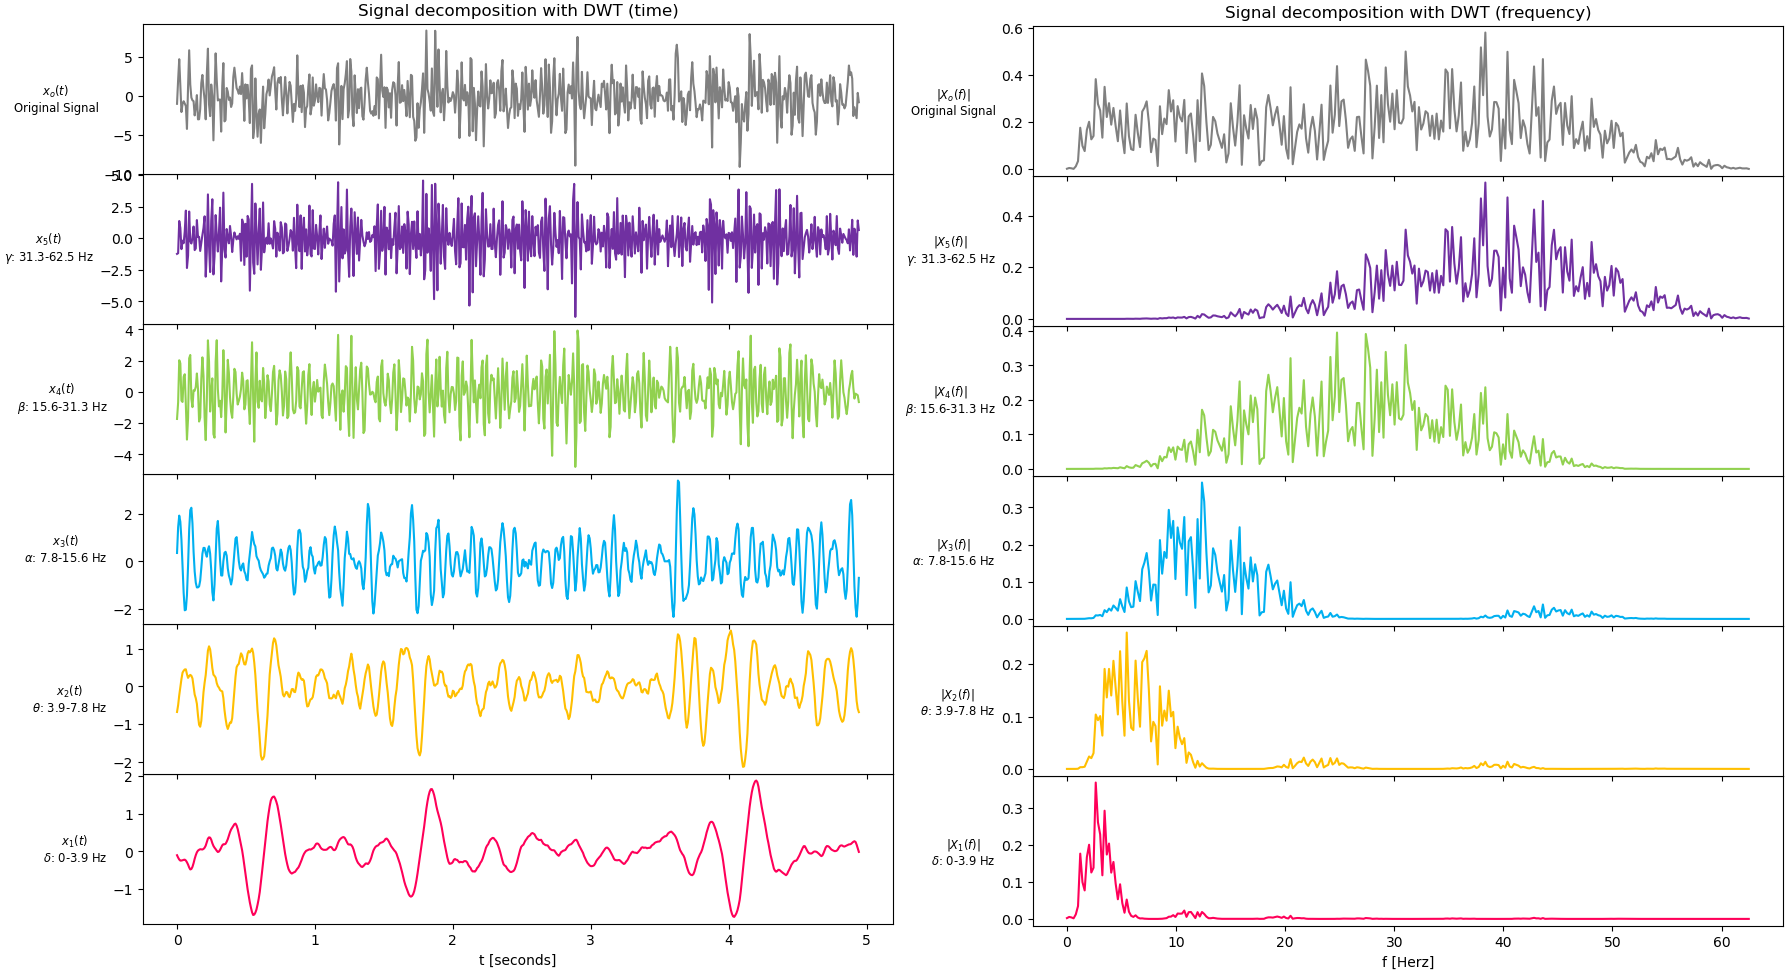
\includegraphics[width=\linewidth]{Figures/DWT_time_freq.png}
	\centering
	\caption{Signal decomposition with DWT.}
	\label{Fig: DWT_freq_time}
\end{figure}

It is noticeable that the concentration of energy vary among sub-bands and time intervals. However, in both cases of using DWT, the energy is more concentrated in $\beta$ and $\gamma$ sub-bands, even though the more detailed decompositions by using WPT show more dispersion of energy. For the class \textit{/iy/}, such dispersion was more notable than for the class \textit{/m/} by presenting energy concentrations varying from 2 to 50 Hz along the timesteps.\\

Due to that, each wavelet approach presents different decompositions of the signals, and as result, different feature vectors are built. In consequence, it was reasonable to compare the classification performance achieved with both wavelet approaches.\\

In order to remark their differences, Figures \ref{Fig: DWT_freq_time} and \ref{Fig: WPT_freq_time} show the signal decomposition applying DWT and WPT, respectively, of the same example from Figure \ref{Fig: Wavelet_freq_time} when the subject imagined the class \textit{/iy/}.\\

The first plot columns show the signal in continuous time followed by each resulting wavelet coefficients set (distinguished by the same sub-band colors of Figures \ref{Fig: Wavelet_decomp} and \ref{Fig: Wavelet_freq_time}). While the second plot columns present their corresponding spectral components computed with the FFT. In the case of DWT spectral plots (Figure \ref{Fig: DWT_freq_time}), it is obvious the band limits of each decomposition with just some small components overlapped in the borderlines of the bands. This effect is notable between $\alpha$ and $\beta$ sub-bands, as well as $\beta$ and $\gamma$ sub-bands.\\

On the other hand, it can be noticed in WPT spectral plots (Figure \ref{Fig: WPT_freq_time}) some components present in sub-bands distant from the band limits of the corresponding decomposition. This phenomenon is notable in some $\beta$ and $\gamma$ sub-bands. (for example in the $\beta$ sub-bands 19.5-23.4 Hz and 23.4-27.3 Hz, as well as in the $\gamma$ sub-bands 50.8-54.7 Hz and 54.7-58.6 Hz) However, such components have less magnitude compared with those concentrated in the sub-band associated with the decomposition.\\

\begin{figure}[H]
	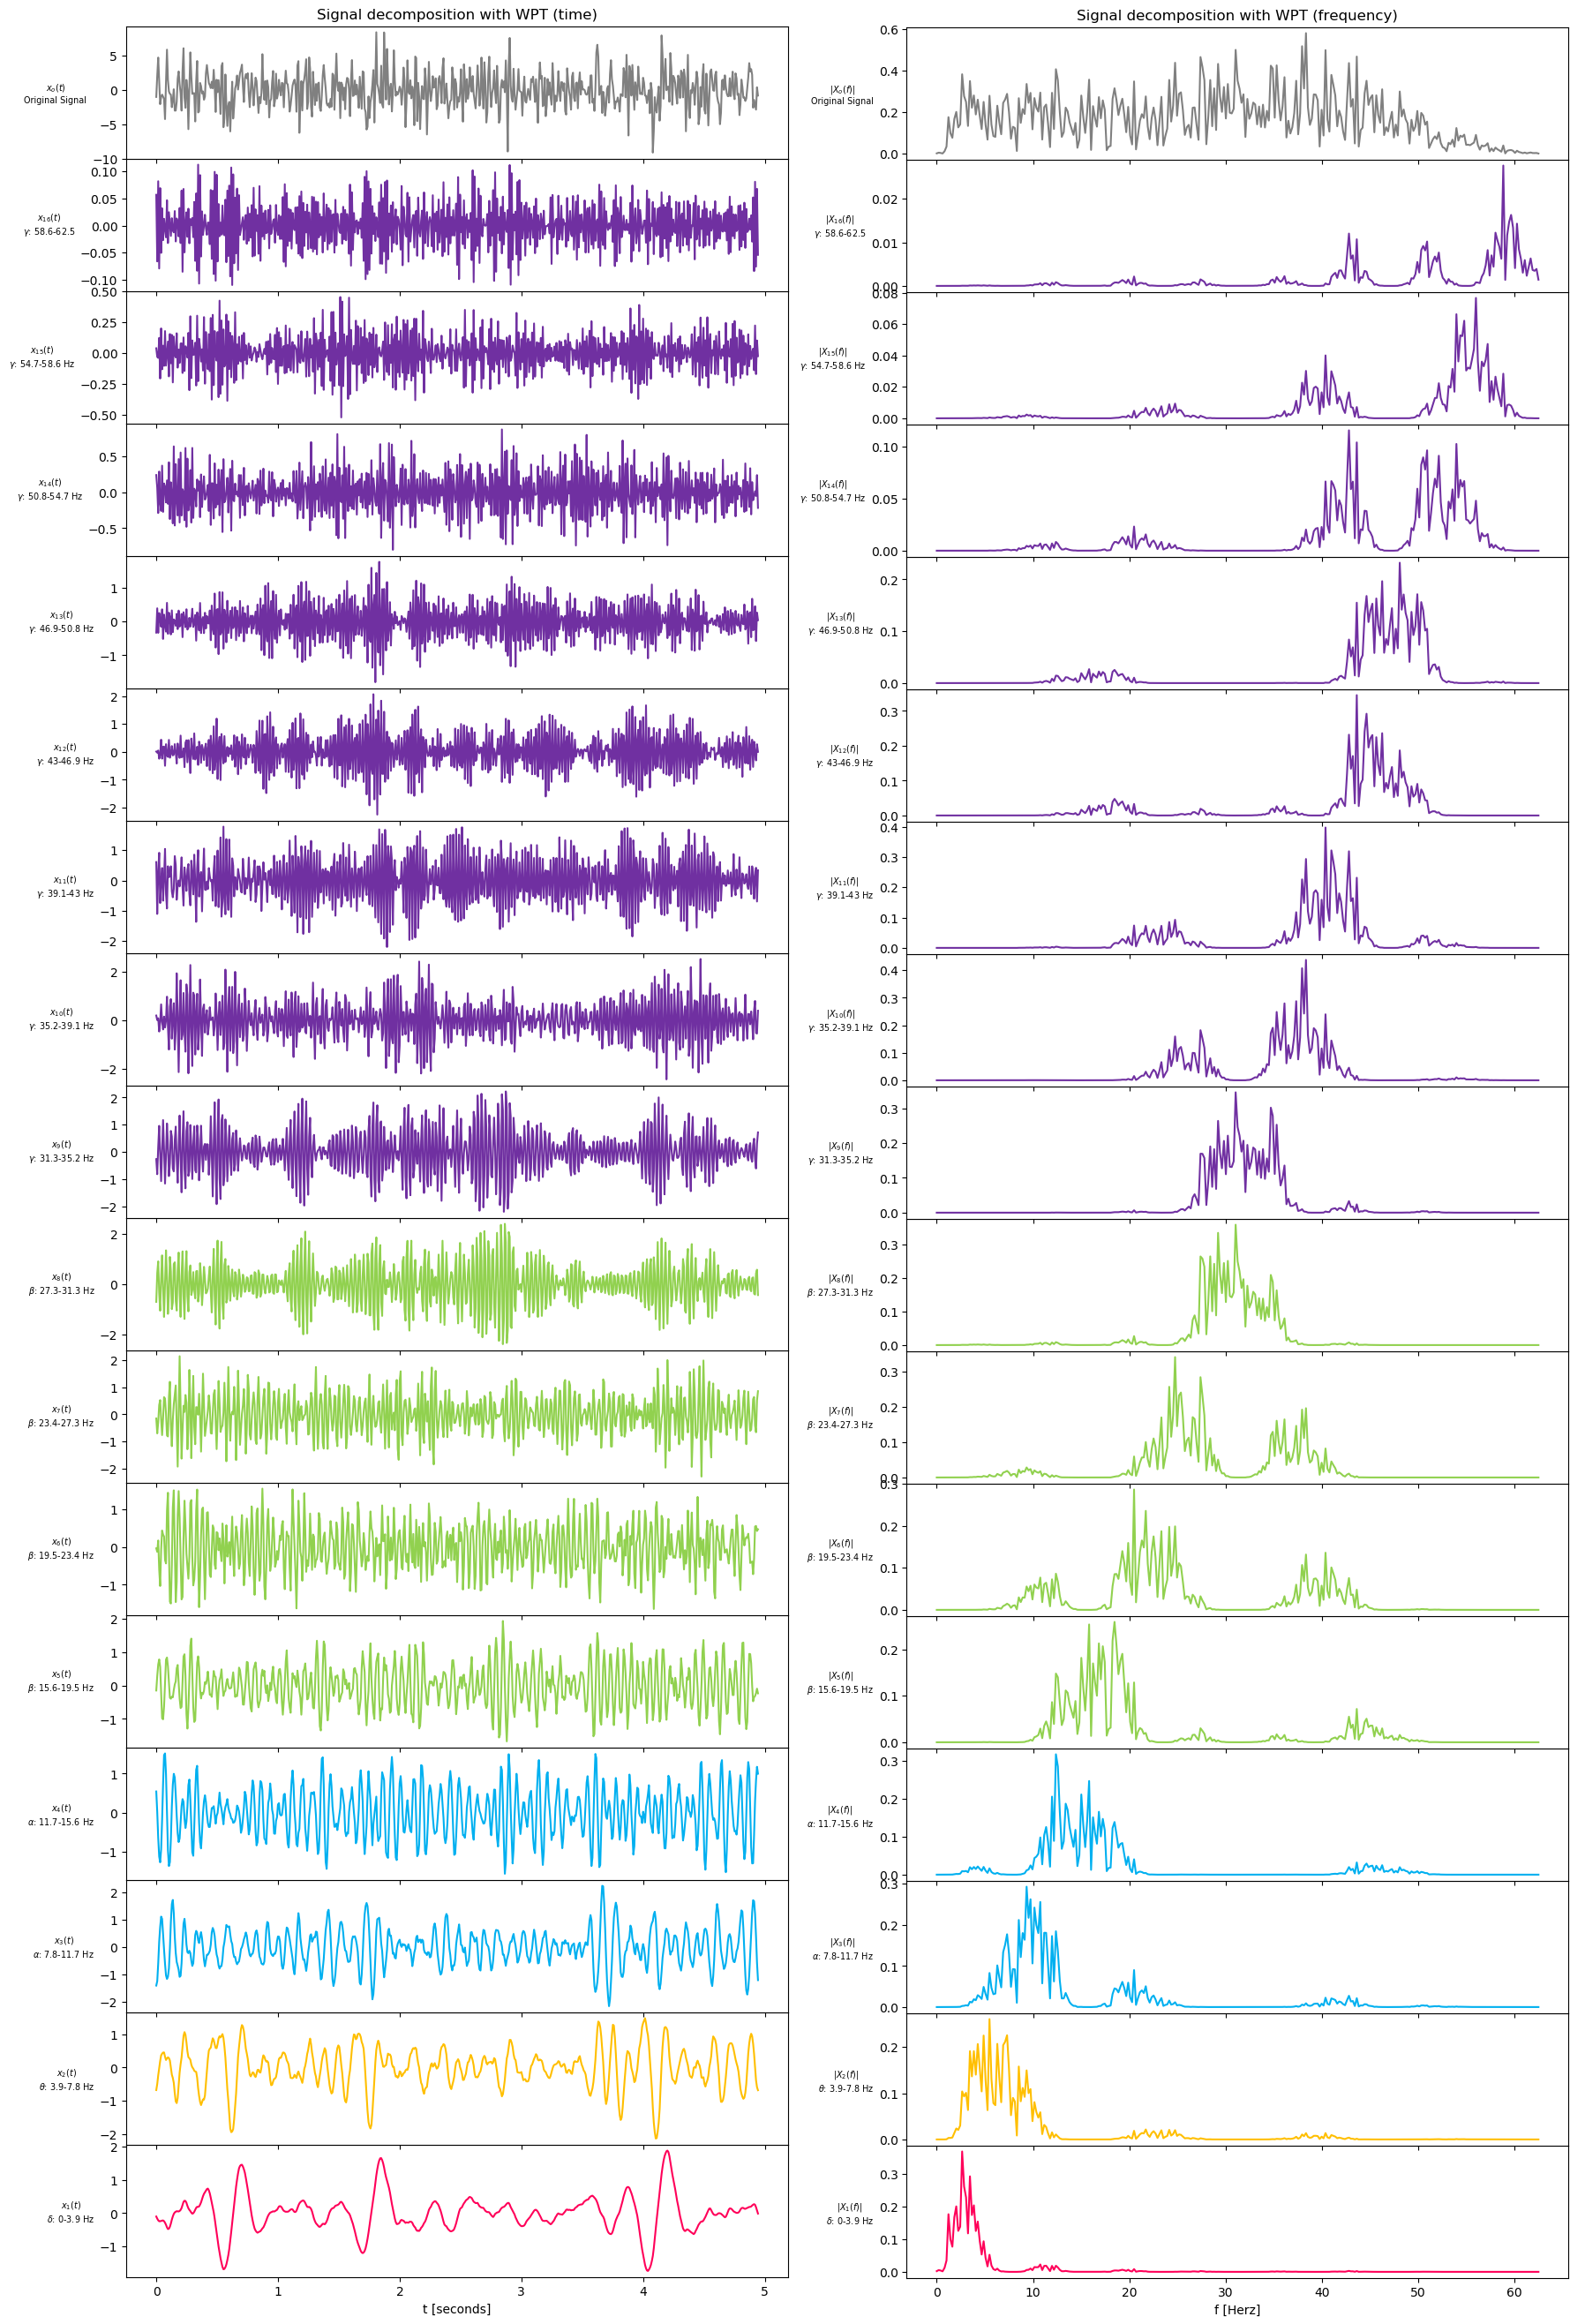
\includegraphics[scale=0.3]{Figures/WPT_time_freq.png}
	\centering
	\caption{Signal decomposition with WPT.}
	\label{Fig: WPT_freq_time}
\end{figure}

\subsubsection{Feature extraction}

\begin{table}[h!]
	\caption{Features extracted (and their identifiers) based on \cite{d2003epileptic} and proposed subset highlighted.}
	\centering
	\begin{tabular}{|c|c|c|c|c|c|}\hline
		\textbf{ID}&\textbf{Name}&\textbf{ID}&\textbf{Name}&\textbf{ID}&\textbf{Name}\\\hline
		$F_{1}$&Mean&$F_{2}$&Mean(Abs)&$F_{3}$&Max\\\hline
		$F_{4}$&Max(Abs)&$F_{5}$&Min&$F_{6}$&Min(Abs)\\\hline
		$F_{7}$&Max+Min&$F_{8}$&Max-Min&$F_{9}$&EHF\\\hline
		\cellcolor{orange}$F_{10}$&\cellcolor{orange}Curvelength&$F_{11}$&Energy&\cellcolor{orange}$F_{12}$&\cellcolor{orange}Avgle\\\hline
		\cellcolor{orange}$F_{13}$&\cellcolor{orange}Spec entr.&$F_{14}$&6th power&$F_{15}$&Integral\\\hline
		$F_{16}$&Stand. Dev&$F_{17}$&Variance&$F_{18}$&Skewness\\\hline
		$F_{19}$&Kurtosis&$F_{20}$&Sum&$F_{21}$&Median\\\hline
	\end{tabular}
	\label{Table: Feature_Extraction}
\end{table}

The same framing procedure, as in \cite{zhao2015classifying}, was followed to extract features over the processed signals (trimmed signals in the case of overt speech and wavelet coefficients in the case of imagined speech). This procedure consisted of framing each signal by segments of approximately 10\% of their lengths and with an overlap of 50\% between each segment, resulting in 19 segments per signal.\\

Then, the features indicated in Table \ref{Table: Feature_Extraction} were computed on every segment. These features were proposed in \cite{d2003epileptic}, and all of them were used in \cite{zhao2015classifying,zhao2013combining}. Apart from computing those 21 features, a subset of three features were selected as a proposal to perform independent classification experiments and compare the performance achieved with both feature sets.\\

The three selected features are highlighted in Table \ref{Table: Feature_Extraction} and they were selected because of their following characteristics defined in \cite{d2003epileptic}:\\

\begin{itemize}
	\item \underline{Curve length (CL)}: It is useful for observing amplitude and frequency changes and dimensionality of the signal. It is defined with the following equation:
	
	\begin{equation}
	\label{Eq: Curve_Length}
	CL_{\ell}=\sum_{m=0}^{M-1}\lvert x[m-1]-x[m]\lvert
	\end{equation}
	
	Where $ M $ is the total number of points in the $ \ell $ segment and $ x[m] $ is the sample point value in $ m $, considering 0 de first position in the segment and $ M-1 $ the last.
	
	\item \underline{Average Nonlinear Energy (ANE)}: It is a measure of energy proportional to both signal amplitude and frequency. This feature is defined as:
	
	\begin{equation}
	\label{Eq: Avg_Nonlinear_Energy}
	ANE_{\ell}=\frac{1}{M}\sum_{m=0}^{M-1}NE[m]
	\end{equation}
	
	From where $ NE[m] $ is defined as:
	
	\begin{equation}
	\label{Eq: Nonlinear_Energy}
	NE[m]=\left\{\begin{array}{lcl}
	x^{2}[m]-x[m-1]x[m+1] & \mbox{if} & 0<m<M-1\\
	&   &   \\
	0 & \mbox{otherwise} & 
	\end{array}\right.
	\end{equation}
	
	In \cite{d2003epileptic} it is specified that a Hanning window must be weighted with all the $ M $ values of $ NE $. However, none window was applied over $ NE $ values for this work, like in \cite{zhao2015classifying,zhao2013combining}.
	
	\item \underline{Spectral Entropy (SE)}: This feature quantifies regularity and order in the signal with the following equation:
	
	\begin{equation}
	\label{Eq: Spectral_Entropy}
	SE_{\ell}=\sum_{\kappa=0}^{M-1}P[\kappa]\log_{2}\{P[\kappa]\}
	\end{equation}
	
	Then, $ P[\kappa] $ is defined as:
	
	\begin{equation}
	\label{Eq: Spectrum_Prob}
	P[\kappa]=\frac{\mid X[\kappa]\mid^{2}}{MF_{s}}, 0\leq\kappa\leq M-1
	\end{equation}
	
	Where $ X $ is the Fourier transform of the signal $ x $ computed with the FFT of M points.
	
\end{itemize}

It is important to remark that the database also has the feature vectors extracted from the preprocessed signals (those after applying the BPF) in files named \textit{all\underline{ }features\underline{ }noIca.mat} and the computation of these features was reproduced based on the definitions of \cite{d2003epileptic}. This reproduction was made to implement the feature extraction step in a DSP for a course.\\

Nevertheless, some of the reproduced feature values differed from those of the database. For example, the spectral entropy and the curve length presented higher values in the database compared with the reproduced values. Besides, these and some other features presented higher values than the rest in the database, which was the motivation to applied a selected normalization in \cite{yazaed} for such features.\\

Due to the discrepancy and high values, the code provided by the University of Toronto was revised and compared with the definitions in \cite{d2003epileptic}. After this revision, it was noticed that the features with such problems, which were stored in the database and used in \cite{zhao2015classifying,zhao2013combining,yazaed}, were wrongly implemented. For this work, the features were computed with the new implementation based on the definitions in \cite{d2003epileptic}.\\

As mentioned before, the framing procedure for this work was similar to that in \cite{zhao2015classifying}. In the case of overt speech, the resulting 19 sequential temporal sub-vectors, each formed by the 3 or 21 features extracted from each segment, represent a whole static feature vector to feed any classifier in this approach.\\

However, for imagined speech, each temporal sub-vector is formed by the 3 or 21 features from each wavelet coefficient set. This process is represented in Figure \ref{Fig: DWT_Framing} with the 5 coefficient sets obtained after applying DWT. Each pair of dashed red or black vertical lines indicates the interval in which the $ L $ features of the $ M_{\ell} $ temporal sub-vector were extracted.\\

\begin{figure}[h!]
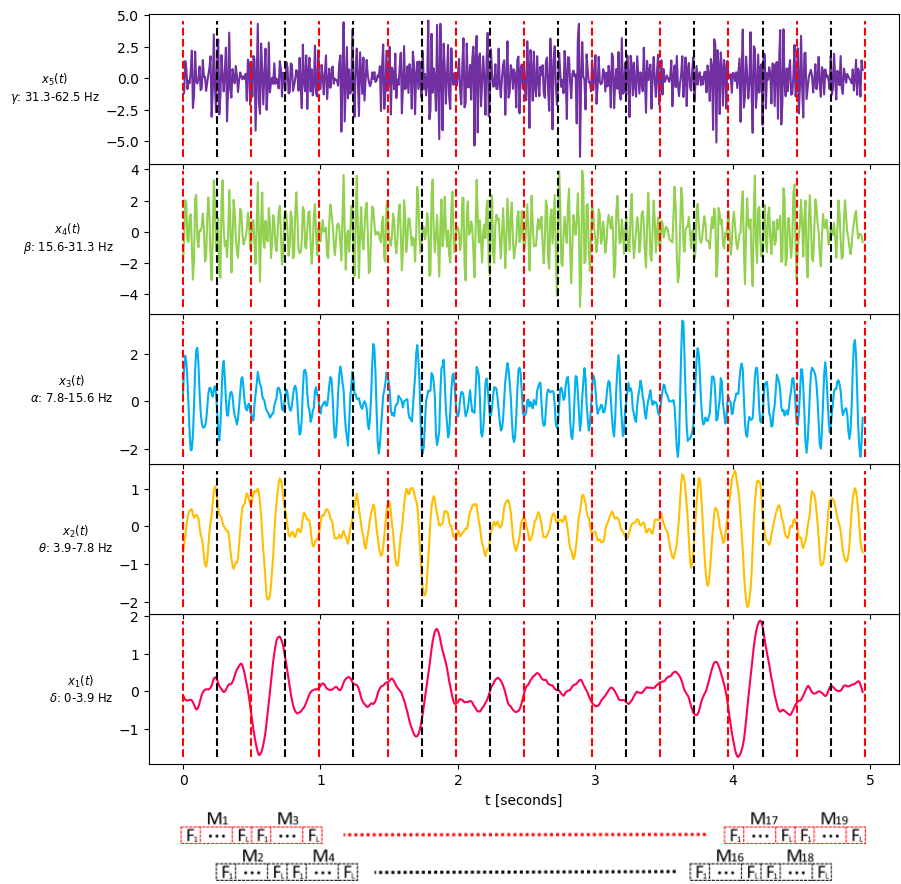
\includegraphics[width=\linewidth]{Figures/DWT_Framing.png}
\centering
\caption{Signal framing from DWT decomposition.}
\label{Fig: DWT_Framing}
\end{figure}

\begin{figure}[h!]
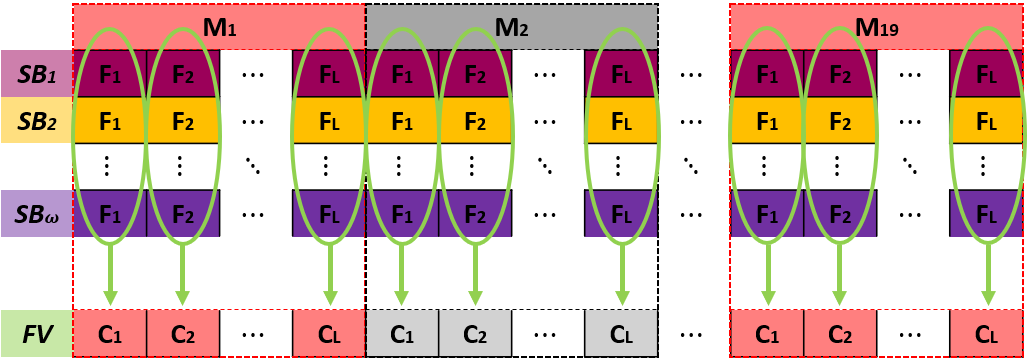
\includegraphics[width=\linewidth]{Figures/PCA.png}
\centering
\caption{PCA over features by wavelet coefficient sub-band.}
\label{Fig: PCA}
\end{figure}

Nonetheless, using temporal sub-vectors from all the coefficient sets would produce feature vectors of high dimensionality, which involves more computation in the classification step. For example, in the simplest case, 3 features and applying DWT, the feature vector dimension would be 285. Whereas, for the most complex case, 21 features and applying WPT, would be of 6384. This dimension variabilities would also require an architecture per case for the MLP since the number of hidden neurons depends on the input dimensions.\\

For this problem, a PCA was performed over each feature. This method reduced and fixed the dimensionality of feature vectors among both wavelet approaches (DWT and WPT). Figure \ref{Fig: PCA} summarizes the processes involved in the PCA methodology applied in this work. The first step consisted of standardizing each feature across all the $ \omega $ sub-bands $ SB $ (i.e., by columns according to the green ovals in Figure \ref{Fig: PCA}). This step is crucial because PCA is sensible to feature scales.\\

According to \cite{pca}, if the data is not standardized, PCA might determine that the direction of maximal variance more closely correspond with the feature with highest scale values, which could not be necessarily true.\\

After standardization, the PCA components were computed across the $ SB $ sub-bands (again, this is indicated with the green ovals in Figure \ref{Fig: PCA}). Here, the $ L $ features from each segment represented the observations, while the sub-bands were the $ \omega $ variables. This process generated a set of components per feature (or observation), from which just the component with most variance was selected to build each temporal sub-vector of the resulting $ FV $ vector represented in Figure \ref{Fig: PCA}\\

The selected component's variances when using 3 and 21 features as observations are summarized in Table \ref{Table: CV_3feats} and \ref{Table: CV_21feats}, respectively. The values in the tables represent the average $ \pm $ the variance computed across all the samples for the specified binary set, segment, and wavelet approach for \textit{FC6} channel data.\\

It can be noticed that the selected components by using 3 features (Table \ref{Table: CV_3feats}) had, on average, variances above 97\%, which means that they contained most of the information when data was reduced. On the other hand, the selected components by using 21 features (Table \ref{Table: CV_21feats}) conserved, on average, 94\% of the information in the best case of DWT, which was reduced when using WPT. This means that PCA was more inconsistent for 21 features than for 3 features across all the binary sets, frames and wavelet approaches.\\

It is also important to mention that previously another approach was performed to reduce the size of feature vectors from imagined speech signals. This approach consisted of correlating the feature vector from each EEG signal with each feature vector from the resulting wavelet coefficient sets of the same signal. Then, based on the resulting ranking, just the most correlated coefficient sets were selected from all the decompositions.\\

In Figure \ref{Fig: Correlation} is represented this selection process with all the samples used in this work. \small$ \nu_{O }$ represent the feature vectors from the EEG signal and $ \nu_{SB} $  signify a specific wavelet coefficients set. Also, $\rho$ is the Spearman correlation between each pair of vectors.\\

\begin{table}[h!]
	\centering
	\caption{Average Variance of selected components across wavelet approaches and segments using 3 features.}
	\scalebox{0.7}{
	\begin{tabular}{|*{9}{c|}}
		\cline{2-9}
		\multicolumn{1}{c|}{\multirow{1}{*}{}}& \multicolumn{4}{c|}{\textbf{DWT}}       & \multicolumn{4}{c|}{\textbf{WPT}} \\\hline
		\textbf{CV}    & \textbf{-Nasal} & \textbf{+Nasal} & \textbf{-Bilabial} & \textbf{+Bilabial} & \textbf{-Nasal} & \textbf{+Nasal} & \textbf{-Bilabial} & \textbf{+Bilabial} \\\hline
		\textbf{1}     & 98.48$ \pm $2.83 & 98.04$ \pm $3.34 & 98.23$ \pm $3.04 & 98.47$ \pm $3.03 & 99.37$ \pm $1.28 & 99.17$ \pm $1.53 & 99.26$ \pm $1.36 & 99.35$ \pm $1.41 \\\hline
		\textbf{2}     & 98.1$ \pm $3.56 & 98.24$ \pm $2.94 & 98.28$ \pm $3.11 & 97.95$ \pm $3.7 & 99.21$ \pm $1.54 & 99.26$ \pm $1.34 & 99.29$ \pm $1.31 & 99.12$ \pm $1.69 \\\hline
		\textbf{3}     & 97.97$ \pm $3.49 & 98.27$ \pm $2.74 & 98.28$ \pm $2.95 & 97.75$ \pm $3.65 & 99.14$ \pm $1.56 & 99.29$ \pm $1.13 & 99.29$ \pm $1.24 & 99.03$ \pm $1.66 \\\hline
		\textbf{4}     & 98.18$ \pm $3.34 & 98.29$ \pm $3.09 & 98.32$ \pm $3.23 & 98.05$ \pm $3.28 & 99.25$ \pm $1.42 & 99.29$ \pm $1.34 & 99.32$ \pm $1.35 & 99.19$ \pm $1.45 \\\hline
		\textbf{5}     & 98.39$ \pm $3.04 & 98.58$ \pm $2.61 & 98.56$ \pm $2.85 & 98.31$ \pm $2.96 & 99.34$ \pm $1.33 & 99.36$ \pm $1.43 & 99.36$ \pm $1.42 & 99.31$ \pm $1.27 \\\hline
		\textbf{6}     & 98.44$ \pm $3.03 & 98.59$ \pm $2.63 & 98.48$ \pm $2.99 & 98.51$ \pm $2.68 & 99.37$ \pm $1.26 & 99.34$ \pm $1.45 & 99.33$ \pm $1.46 & 99.41$ \pm $1.09 \\\hline
		\textbf{7}     & 98.59$ \pm $2.76 & 98.69$ \pm $2.71 & 98.71$ \pm $2.74 & 98.49$ \pm $2.74 & 99.42$ \pm $1.21 & 99.45$ \pm $1.16 & 99.46$ \pm $1.18 & 99.39$ \pm $1.22 \\\hline
		\textbf{8}     & 98.49$ \pm $3.14 & 98.69$ \pm $2.45 & 98.62$ \pm $3.02 & 98.47$ \pm $2.69 & 99.36$ \pm $1.44 & 99.48$ \pm $0.97 & 99.41$ \pm $1.35 & 99.39$ \pm $1.17 \\\hline
		\textbf{9}     & 98.49$ \pm $3.07 & 98.85$ \pm $2.25 & 98.76$ \pm $2.7 & 98.39$ \pm $2.93 & 99.36$ \pm $1.43 & 99.52$ \pm $0.95 & 99.47$ \pm $1.29 & 99.34$ \pm $1.25 \\\hline
		\textbf{10}    & 98.61$ \pm $2.84 & 98.78$ \pm $2.41 & 98.86$ \pm $2.56 & 98.35$ \pm $2.86 & 99.41$ \pm $1.29 & 99.48$ \pm $1.14 & 99.51$ \pm $1.23 & 99.31$ \pm $1.25 \\\hline
		\textbf{11}    & 98.59$ \pm $2.52 & 98.81$ \pm $2.39 & 98.87$ \pm $2.21 & 98.35$ \pm $2.85 & 99.43$ \pm $1.01 & 99.49$ \pm $1.08 & 99.54$ \pm $0.91 & 99.31$ \pm $1.22 \\\hline
		\textbf{12}    & 98.57$ \pm $2.92 & 98.85$ \pm $2.28 & 98.77$ \pm $2.54 & 98.51$ \pm $2.95 & 99.39$ \pm $1.36 & 99.52$ \pm $1 & 99.47$ \pm $1.21 & 99.38$ \pm $1.29 \\\hline
		\textbf{13}    & 98.51$ \pm $3.17 & 98.63$ \pm $2.53 & 98.53$ \pm $2.92 & 98.58$ \pm $3.01 & 99.34$ \pm $1.56 & 99.43$ \pm $1.1 & 99.36$ \pm $1.44 & 99.39$ \pm $1.37 \\\hline
		\textbf{14}    & 98.38$ \pm $3.24 & 98.67$ \pm $2.48 & 98.46$ \pm $3.04 & 98.53$ \pm $2.88 & 99.34$ \pm $1.39 & 99.46$ \pm $0.99 & 99.37$ \pm $1.27 & 99.41$ \pm $1.23 \\\hline
		\textbf{15}    & 98.61$ \pm $2.8 & 98.57$ \pm $2.76 & 98.54$ \pm $2.8 & 98.69$ \pm $2.76 & 99.42$ \pm $1.24 & 99.39$ \pm $1.29 & 99.41$ \pm $1.17 & 99.42$ \pm $1.39 \\\hline
		\textbf{16}    & 98.73$ \pm $2.69 & 98.69$ \pm $2.72 & 98.69$ \pm $2.75 & 98.77$ \pm $2.62 & 99.46$ \pm $1.22 & 99.44$ \pm $1.27 & 99.45$ \pm $1.22 & 99.47$ \pm $1.26 \\\hline
		\textbf{17}    & 98.81$ \pm $2.52 & 98.68$ \pm $2.69 & 98.75$ \pm $2.48 & 98.76$ \pm $2.77 & 99.51$ \pm $1.11 & 99.47$ \pm $1.05 & 99.48$ \pm $1.09 & 99.51$ \pm $.1.08 \\\hline
		\textbf{18}    & 99$ \pm $2.09 & 98.77$ \pm $2.44 & 98.86$ \pm $2.46 & 99.02$ \pm $1.77 & 99.6$ \pm $0.84 & 99.49$ \pm $1.12 & 99.53$ \pm $1.09 & 99.61$ \pm $0.66 \\\hline
		\textbf{19}    & 98.83$ \pm $2.01 & 98.75$ \pm $2.45 & 98.69$ \pm $2.43 & 98.96$ \pm $1.7 & 99.54$ \pm $0.74 & 99.47$ \pm $1.14 & 99.47$ \pm $1.04 & 99.59$ \pm $0.63 \\\hline
	\end{tabular}%
	}
	\label{Table: CV_3feats}%
\end{table}%

\begin{table}[h!]
	\centering
	\caption{Average Variance of selected components across wavelet approaches and segments using 21 features.}
	\scalebox{0.665}{
	\begin{tabular}{|*{9}{c|}}
		\cline{2-9}
		\multicolumn{1}{c|}{\multirow{1}{*}{}}& \multicolumn{4}{c|}{\textbf{DWT}}       & \multicolumn{4}{c|}{\textbf{WPT}} \\\hline
		\textbf{CV}    & \textbf{-Nasal} & \textbf{+Nasal} & \textbf{-Bilabial} & \textbf{+Bilabial} & \textbf{-Nasal} & \textbf{+Nasal} & \textbf{-Bilabial} & \textbf{+Bilabial} \\\hline
		\textbf{1}     & 80.92$ \pm $16.55 & 81.59$ \pm $14 & 98.37$ \pm $5.75 & 98.17$ \pm $6.16 & 79.17$ \pm $8.75 & 79.65$ \pm $9.37 & 74.88$ \pm $10.23 & 80.4$ \pm $11.28 \\\hline
		\textbf{2}     & 81.69$ \pm $15.62 & 82.01$ \pm $13.54 & 98.33$ \pm $6.05 & 97.71$ \pm $7.24 & 79.46$ \pm $8.71 & 79.21$ \pm $9.16 & 73.36$ \pm $8.9 & 79.04$ \pm $10.59 \\\hline
		\textbf{3}     & 81.52$ \pm $14.83 & 82.17$ \pm $13.66 & 98.39$ \pm $6.22 & 97.47$ \pm $7.64 & 79.60$ \pm $8.76 & 79.01$ \pm $8.37 & 73.09$ \pm $9.19 & 78.68$ \pm $10.78 \\\hline
		\textbf{4}     & 80.66$ \pm $15.93 & 82.82$ \pm $13.75 & 96.99$ \pm $8.26 & 97.13$ \pm $8.14 & 79.76$ \pm $8.69 & 79.60$ \pm $8.97 & 73.02$ \pm $9.41 & 78.54$ \pm $10.72 \\\hline
		\textbf{5}     & 80.5$ \pm $15.39 & 82.48$ \pm $13.49 & 96.72$ \pm $8.33 & 96.98$ \pm $8.72 & 79.75$ \pm $8.51 & 79.89$ \pm $9.21 & 72.78$ \pm $9.39 & 77.94$ \pm $10.74 \\\hline
		\textbf{6}     & 81.09$ \pm $14.69 & 80.73$ \pm $14.45 & 96.29$ \pm $9.39 & 96.68$ \pm $8.82 & 79.71$ \pm $8.55 & 79.87$ \pm $9.38 & 72.65$ \pm $9.09 & 77.73$ \pm $10.82 \\\hline
		\textbf{7}     & 80.69$ \pm $14.57 & 80.62$ \pm $14.09 & 95.97$ \pm $10.49 & 96.36$ \pm $10.04 & 80.5$ \pm $8.85 & 79.69$ \pm $9.92 & 72.82$ \pm $9.05 & 77.44$ \pm $10.76 \\\hline
		\textbf{8}     & 81.32$ \pm $14.43 & 80.72$ \pm $13.99 & 96.02$ \pm $10.09 & 96.36$ \pm $9.17 & 80.32$ \pm $9.14 & 80.12$ \pm $9.17 & 72.88$ \pm $9.19 & 78.18$ \pm $10.43 \\\hline
		\textbf{9}     & 81.55$ \pm $14.56 & 81.25$ \pm $13.52 & 95.89$ \pm $10.06 & 96.76$ \pm $8.77 & 79.98$ \pm $9.21 & 80.34$ \pm $8.85 & 72.42$ \pm $9.15 & 78.36$ \pm $10.24 \\\hline
		\textbf{10}    & 80.64$ \pm $14.49 & 81.47$ \pm $13.2 & 95.69$ \pm $10.34 & 97.05$ \pm $7.79 & 79.95$ \pm $9.66 & 80.39$ \pm $8.76 & 72.51$ \pm $9.14 & 77.89$ \pm $10.61 \\\hline
		\textbf{11}    & 80.39$ \pm $14.46 & 80.55$ \pm $14.09 & 95.59$ \pm $10.39 & 96.32$ \pm $9.32 & 80.72$ \pm $9.27 & 80.69$ \pm $8.73 & 72.49$ \pm $9.13 & 77.72$ \pm $10.76 \\\hline
		\textbf{12}    & 80.53$ \pm $14.14 & 80.36$ \pm $13.56 & 95.51$ \pm $10.64 & 95.85$ \pm $10.32 & 80.89$ \pm $8.93 & 80.2$ \pm $9.13 & 72.21$ \pm $0.09 & 77.4210.87 \\\hline
		\textbf{13}    & 80.88$ \pm $14.59 & 81.03$ \pm $13 & 95.52$ \pm $10.45 & 95.75$ \pm $10.58 & 80.61$ \pm $9.08 & 79.71$ \pm $9.39 & 72.32$ \pm $9.09 & 77.23$ \pm $10.81 \\\hline
		\textbf{14}    & 81.05$ \pm $13.89 & 80.55$ \pm $14.05 & 95.48$ \pm $10.85 & 95.92$ \pm $9.89 & 80.66$ \pm $9.13 & 79.95$ \pm $9.23 & 72.25$ \pm $8.99 & 76.91$ \pm $10.69 \\\hline
		\textbf{15}    & 80.86$ \pm $13.71 & 79.75$ \pm $14.61 & 95.01$ \pm $11.18 & 96.2$ \pm $10.51 & 80.91$ \pm $9.05 & 80.19$ \pm $9.39 & 72.23$ \pm $8.89 & 76.59$ \pm $10.68 \\\hline
		\textbf{16}    & 80.76$ \pm $14.55 & 79.43$ \pm $14.62 & 95.15$ \pm $11.21 & 94.54$ \pm $11.56 & 80.75$ \pm $9.17 & 80.41$ \pm $9.48 & 72.46$ \pm $8.79 & 76.91$ \pm $10.75 \\\hline
		\textbf{17}    & 80.14$ \pm $14.78 & 79.02$ \pm $14.89 & 94.44$ \pm $12.33 & 94.07$ \pm $12.09 & 80.86$ \pm $8.79 & 80.76$ \pm $9.36 & 72.34$ \pm $8.94 & 76.89$ \pm $10.47 \\\hline
		\textbf{18}    & 80.09$ \pm $14.93 & 80.41$ \pm $14.43 & 94.09$ \pm $12.85 & 94.65$ \pm $11.89 & 80.66$ \pm $9.05 & 80.37$ \pm $9.02 & 72.45$ \pm $8.78 & 76.66$ \pm $10.18 \\\hline
		\textbf{19}    & 79.22$ \pm $14.5 & 80.33$ \pm $14.63 & 95.01$ \pm $11.25 & 96.26$ \pm $9.14 & 80.2$ \pm $8.93 & 80.05$ \pm $8.73 & 73.61$ \pm $10.25 & 77.98$ \pm $10.98 \\\hline
	\end{tabular}%
	}
	\label{Table: CV_21feats}%
\end{table}%

\begin{figure}[h!]
\centering
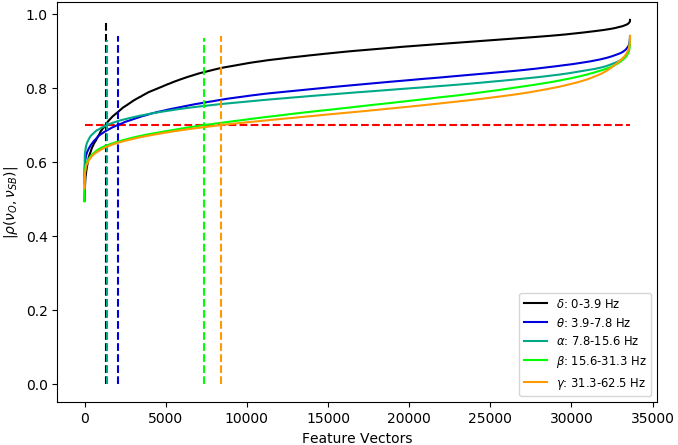
\includegraphics[width=\linewidth]{Figures/Correlation.png}
\caption{Spearman correlation using DWT and 3 features.}
\label{Fig: Correlation}
\end{figure}

Besides, each straight colored curve represents all the absolute correlation coefficient values sorted in ascending order as a result of correlating all the $ \nu_{SB} $ vectors (associated with sub-bands distinguished in the legend) with their corresponding \small$ \nu_{O }$ vector.\\

Also, the horizontal dashed red line is a threshold fixed in 0.7, and the vertical dashed lines indicate the points where each corresponding correlation curve crosses the threshold. Just the three $ \nu_{SB} $ vectors with more amount of correlation coefficients above the threshold were selected for the classification step.\\

In Figure \ref{Fig: Correlation}, where DWT and 3 features were computed, the three $ \nu_{SB} $ vectors  correspond to $ \theta $, $ \delta $,and $ \alpha $ sub-bands. Indeed, for the other cases (21 features and DWT, 3 or 21 features and WPT) the corresponding sub-bands of the selected vectors were the same. In Table \ref{Table: Correlation} are shown, for all the cases (wavelet approach and computed features), the ranking, the associated sub-bands with the wavelet coefficient sets, their corresponding range in Hz, and the percentage of correlation coefficients (from a total of 33604) above the threshold per case. Also, the three selected feature vectors are highlighted in Table \ref{Table: Correlation}, which were selected due to their notorious percentage of correlation coefficients comparing with the rest of the feature vectors.\\

This process was done with Kendall and Pearson correlation too. However, the results obtained with Kendall correlation were the worst, from which in most of the cases the best sub-band correlated obtained 76.67\% of correlation coefficients above the threshold.\\

While for Pearson correlation, apart of obtaining similar results as with Kendall correlation, was necessary to carry the Kolmogorov-Smirnoff test to decide if the correlation values were significant, i.e. if $ \nu_{SB} $ and \small$ \nu_{O }$ came from the same continuous distribution (H$ _{o} $) or not (H$ _{a} $). The Kolmogorov-Smirnoff test was carried with a 5\% significance level, which rejected H$ _{o} $ for all $ \nu_{SB} $ and \small$ \nu_{O }$ pairs.\\

\begin{table}[h!]
	\centering
	\caption{Spearman correlation rankings per case and selected sub-bands}
	\scalebox{0.85}{
	\begin{tabular}{|*{8}{c|}}
		\cline{3-8}
		\multicolumn{2}{c|}{\multirow{1}{*}{}} & \multicolumn{3}{c|}{\textbf{3 features}} & \multicolumn{3}{c|}{\textbf{21 features}} \\\cline{2-8}
		\multicolumn{1}{c|}{\multirow{1}{*}{}} & \textbf{Rank} & \textbf{Subband} & \textbf{Range} & \textbf{Percentage} & \textbf{Subband} & \textbf{Range} & \textbf{Percentage} \\\hline
		\multirow{5}{*}{\begin{sideways}\textbf{DWT}\end{sideways}} & \cellcolor{orange}1     & \cellcolor{orange}$\delta$ & \cellcolor{orange}0-3.9 & \cellcolor{orange}96.14 & \cellcolor{orange}$\delta$ & \cellcolor{orange}0-3.9 & \cellcolor{orange}44.93 \\\cline{2-8}
		& \cellcolor{orange}2     & \cellcolor{orange}$\alpha$ & \cellcolor{orange}7.8-15.6 & \cellcolor{orange}95.91 & \cellcolor{orange}$\theta$ & \cellcolor{orange}3.9-7.8 & \cellcolor{orange}34.5 \\\cline{2-8}
		& \cellcolor{orange}3     & \cellcolor{orange}$\theta$ & \cellcolor{orange}3.9-7.8 & \cellcolor{orange}93.92 & \cellcolor{orange}$\alpha$ & \cellcolor{orange}7.8-15.6 & \cellcolor{orange}28.07 \\\cline{2-8}
		& 4     & $\beta$ & 15.6-31.3 & 78.07 & $\beta$ & 15.6-31.3 & 19.85 \\\cline{2-8}
		& 5     & $\gamma$ & 31.3-62.5 & 75.03 & $\gamma$ & 31.3-62.5 & 17.48 \\\hline
		\multirow{16}{*}{\begin{sideways}\textbf{WPT}\end{sideways}} & \cellcolor{orange}1     & \cellcolor{orange}$\delta$ & \cellcolor{orange}0-3.9 & \cellcolor{orange}96.39 & \cellcolor{orange}$\delta$ & \cellcolor{orange}0-3.9 & \cellcolor{orange}96.14 \\\cline{2-8}
		& \cellcolor{orange}2     & \cellcolor{orange}$\theta$ & \cellcolor{orange}3.9-7.8 & \cellcolor{orange}95.38 & \cellcolor{orange}$\alpha$ & \cellcolor{orange}7.8-11.7 & \cellcolor{orange}95.91 \\\cline{2-8}
		& \cellcolor{orange}3     & \cellcolor{orange}$\alpha$ & \cellcolor{orange}7.8-11.7 & \cellcolor{orange}90.29 & \cellcolor{orange}$\theta$ & \cellcolor{orange}3.9-7.8 & \cellcolor{orange}93.92 \\\cline{2-8}
		& 4     & $\gamma$ & 31.3-35.2 & 80.63 & $\alpha$ & 11.7-15.6 & 78.07 \\\cline{2-8}
		& 5     & $\beta$ & 27.3-31.3 & 78.9  & $\beta$ & 15.6-19.5 & 75.03 \\\cline{2-8}
		& 6     & $\gamma$ & 35.2-39.1 & 78.35 & $\beta$ & 19.5-23.4 & 74.56 \\\cline{2-8}
		& 7     & $\gamma$ & 39.1-43 & 74.94 & $\beta$ & 27.3-31.3 & 69.29 \\\cline{2-8}
		& 8     & $\beta$ & 23.4-27.3 & 68.02 & $\gamma$ & 31.3-35.2 & 68.25 \\\cline{2-8}
		& 9     & $\alpha$ & 11.7-15.6 & 67.77 & $\beta$ & 23.4-27.3 & 61.86 \\\cline{2-8}
		& 10    & $\beta$ & 15.6-19.5 & 66.21 & $\gamma$ & 35.2-39.1 & 55.21 \\\cline{2-8}
		& 11    & $\beta$ & 19.5-23.4 & 62.95 & $\gamma$ & 39.1-43 & 47.51 \\\cline{2-8}
		& 12    & $\gamma$ & 43-46.9 & 62.18 & $\gamma$ & 43-46.9 & 35.31 \\\cline{2-8}
		& 13    & $\gamma$ & 46.9-50.8 & 54.79 & $\gamma$ & 46.9-50.8 & 25.43 \\\cline{2-8}
		& 14    & $\gamma$ & 50.8-54.7 & 48.89 & $\gamma$ & 58.6-6 & 7.45 \\\cline{2-8}
		& 15    & $\gamma$ & 58.6-6 & 46.54 & $\gamma$ & 50.8-54.7 & 6.52 \\\cline{2-8}
		& 16    & $\gamma$ & 54.7-58.6 & 46.28 & $\gamma$ & 54.7-58.6 & 2.76 \\\hline
	\end{tabular}%
	}
	\label{Table: Correlation}%
\end{table}%

For the reasons exposed above, Kendall and Pearson correlations were discarded. However, although the best percentages were obtained with Spearman correlation, this overall processing step was discarded since the classification using these feature vectors provided poor score values (around 56\% of accuracy on average). These results were obtained with some tests varying MLP and SVM parameters. Nevertheless, based on the scores, it seemed that the classifiers recognized almost always just one class with these feature vectors.\\

\subsubsection{Classification}

Once the feature vectors were built, which were composed of 19 temporal sub-vectors with 3 or 21 features (or components) each, the general architecture for the classification consisted of stablishing one classifier per existing EEG channel (for this work 62). Figure \ref{Fig: Classification_VB} depicts this architecture, where each classifier received as input feature vectors, of 19 $M$-temporal sub-vectors with $L$ features each, from one particular channel. Besides, the classifiers used in this work were the MLP (ANN) and SVM.\\

As a first step, each classifier received just the corresponding training feature vectors to update their parameters (this is the learning step). Therefore,  a validation methodology (which is explained further) was followed to train the 62 classifiers and compute some scores per channel with all the training data. These scores were obtained to register the performance achieved with each classifier. The score types computed were: accuracy, recall, precision, and F1.\\

\begin{figure}[h!]
	\centering
	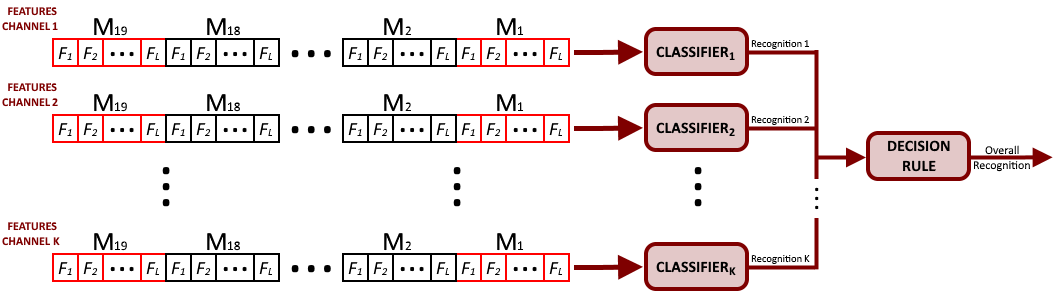
\includegraphics[width=\linewidth]{Figures/Classification_VB.png}
	\caption{Architecture for Vector-based classifiers.}
	\label{Fig: Classification_VB}
\end{figure}

\begin{center}
\scalebox{0.8}{
	\begin{minipage}{0.8\linewidth}
		\begin{algorithm}[H]
			\caption{Channel's selection}
			\label{Algorithm: Channels}
			\hspace*{\algorithmicindent} \textbf{Input:} \\
			\hspace*{\algorithmicindent}\hspace*{\algorithmicindent} $M$: Score matrix \\
			\hspace*{\algorithmicindent}\hspace*{\algorithmicindent} $n$: Number of channels to select \\
			\hspace*{\algorithmicindent} \textbf{Output:} \\
			\hspace*{\algorithmicindent}\hspace*{\algorithmicindent} $\nu$: List of selected channels \\
			\begin{algorithmic}[1]
				\STATE Initialize: $S\leftarrow$ \textbf{0}, $C\leftarrow$ \textbf{0}, list $\nu$
				\FOR{$i=1$ to $u$}{
					\STATE $S_{i} \leftarrow $ \textbf{sort($M_{i}$)}
					\STATE $C_{i} \leftarrow $ \textbf{argsort($M_{i}$)}
				}
				\ENDFOR
				\STATE Flatten $S$ and $C$
				\STATE $\vec{c} \leftarrow $ \textbf{sortscores($S$,$C$)}
				\STATE $i=1$
				\REPEAT
				\IF{$\vec{c}_{i}$ not in $\nu$}
				\STATE Add $\vec{c}_{i}$ to list $\nu$
				\ENDIF
				\STATE $i \leftarrow i+1$
				\UNTIL \textbf{dim($\nu$) $=n$}
			\end{algorithmic}
		\end{algorithm}
	\end{minipage}
}
\end{center}

In the particular case of the MLP, this learning step was performed 20 times with different initializations since this classifier is sensitive to the initial parameter's values. After storing the scores from the 20 initializations, the averages of each score type across all the iterations were computed and stored per channel to register their performance.\\

Next, the second step (named score improvement in Figure \ref{Fig: Diagram}) consisted of selecting just a channel's subset based on the best scores obtained in the previous step. For this step, just one score type was selected as a reference.\\

The Algorithm \ref{Algorithm: Channels} illustrates this process, in which the input matrix $M$ contained the scores and had dimensions of $u$ by $n$ (number of subjects and channels, respectively). Besides, the output list $ \nu $ stored the $n$ channel's identifiers from which were obtained the highest scores. $M$ is a matrix because each row represents the scores obtained across all the channels when all data except subject's data associated with such row were used to train the classifier.\\

\begin{table}[h!]
	\centering
	\caption{Selected channels in \cite{zhao2015classifying,zhao2013combining}, and those selected in this work for overt and imagined speech using MLP and SVM.}
	\scalebox{0.7}{
		\begin{tabular}{|*{11}{c|}}
			\cline{4-11}
			\multicolumn{3}{c|}{\multirow{1}{*}{}} & \multicolumn{4}{c|}{\textbf{Overt speech}} & \multicolumn{4}{c|}{\textbf{Imagined speech}} \\\cline{2-11}
			\multicolumn{1}{c|}{\multirow{1}{*}{}} & \multicolumn{2}{c|}{\textbf{Kara One}} & \multicolumn{2}{c|}{\textbf{MLP}} & \multicolumn{2}{c|}{\textbf{SVM}} & \multicolumn{2}{c|}{\textbf{MLP}} & \multicolumn{2}{c|}{\textbf{SVM}} \\\hline
			\textbf{Ranking} & \textbf{Channel} & \boldmath$\rho$ & \textbf{Channel} & \textbf{F1} & \textbf{Channel} & \textbf{F1}    & \textbf{Channel} & \textbf{F1}    & \textbf{Channel} & \textbf{F1} \\\hline
			\textbf{1}     &  FC6 & 0.3781 &  C3 & 61.9474 & FZ    & 82.9932 &  FC6 & 53.9541 & AF4   & 83.0296 \\\hline
			\textbf{2}     &  FT8 & 0.3758 &  FC6 & 60.5664 & C2    & 82.0485 &  CP5 & 53.5614 & OZ    & 82.0796 \\\hline
			\textbf{3}     &  C5 & 0.3728 & PO3   & 60.3989 & CP6   & 81.7204 & F5    & 51.1207 & P8    & 82.0088 \\\hline
			\textbf{4}     &  CP3 & 0.372 & F4    & 60.377 & TP7   & 76.1885 & FT7   & 50.6732 & PZ    & 82.0088 \\\hline
			\textbf{5}     &  P3 & 0.3696 & C1    & 60.0264 &  CP3 & 74.2852 & C6    & 50.549 & F1    & 82.0088 \\\hline
			\textbf{6}     & T7    & 0.3686 &  CP3 & 59.8149 & O1    & 73.9607 &  FT8 & 50.4072 & AF3   & 82.0088 \\\hline
			\textbf{7}     &  CP5 & 0.3685 & CPZ   & 59.6918 &  P3 & 73.2558 &  C5 & 50.2671 & POZ   & 81.8386 \\\hline
			\textbf{8}     &  C3 & 0.3659 & F5    & 58.9745 & FC4   & 73.1938 & C1    & 50.1141 & FC1   & 81.6886 \\\hline
			\textbf{9}     & CP1   & 0.3626 & FC5   & 58.9437 & CB2   & 71.7073 & FC4   & 49.8666 & CB2   & 81.2775 \\\hline
			\textbf{10}    & C4    & 0.3623 &  C5 & 58.6208 & P2    & 71.6779 & F8    & 49.6962 &  C3 & 81.2775 \\\hline
		\end{tabular}%
	}
	\label{Table: Channel_Selection}%
\end{table}%

Also, $S$ and $C$ represent two matrices (of $u$ by $n$) that store, by row and in descending order, the sorted score values and their channel's identifiers, respectively. After the storage, both matrices were flattened to sort again $C$ based on the values of $S$. Then, the resulting values were stored in $\vec{c}$. Finally, the first $n$ unique values of $\vec{c}$ were added to the output list $\nu$.\\

For this work, the value of $n$ was set to 10. This decision was made to perform experiments comparable with \cite{zhao2015classifying,zhao2013combining}. Additionally, some classification experiments were carried, in which the number of selected channels was varied. After finishing these \linebreak[4]experiments, the best scores were obtained by using 10 channels.\\

On the other hand, the score type used to select a subset of channels was F1. This decision was made again after performing some experiments using the accuracy and F1 scores in the process described in Algorithm \ref{Algorithm: Channels}. The selected channels based on the F1 score provided better performance in the third step than those based on the accuracy score. Besides, it was noticed that the classifiers from the selected channels based on the accuracy classified almost all samples as one particular class.\\

In Table \ref{Table: Channel_Selection} are shown the selected channels and the scores obtained with MLP and SVM classifiers for overt and imagined speech (no wavelet decomposition performed). These channels were also the result of using 3 features and $\pm$Bilabial binary sets. Additionally, the 10 selected channels in \cite{zhao2015classifying,zhao2013combining} are shown in the column Kara One in Table \ref{Table: Channel_Selection}. Notice that the score used there was the Pearson correlation (denoted with the letter $\rho$) between feature vectors from acoustic, and EEG imagined speech signals.\\

Therefore, in Table \ref{Table: Channel_Selection} can be noticed that the resulting selected channels vary among classifiers, mental states, and experimental approaches. Figure \ref{Fig: Channel_Selection} illustrates these \linebreak[4]differences, where it can be seen that for overt speech samples, just one channel (CP3) was common among all the cases. Whereas, for imagined speech samples was not any channel in common. Besides, the best scores were obtained by using SVMs; however, comparing both, Table \ref{Table: Channel_Selection} and Figure \ref{Fig: Channel_Selection}, these selected channels were not common with MLP, neither with \cite{zhao2015classifying,zhao2013combining}.\\

To complement the explanation of Algorithm  \ref{Algorithm: Channels}, in Table \ref{Table: Channel_Selection_Example} is shown the channel selection process of the same case of Table \ref{Table: Channel_Selection} by using an SVM for overt speech. The Scores and Channels represent, respectively, the $S$ and $C$ matrices from the algorithm (once finished the for cycle). Then, the orange row contains the selected channels (those in yellow in $S$ and $C$ matrices), which were selected in the order exposed in the Ranking row.\\

\begin{figure}[h!]
	\centering
	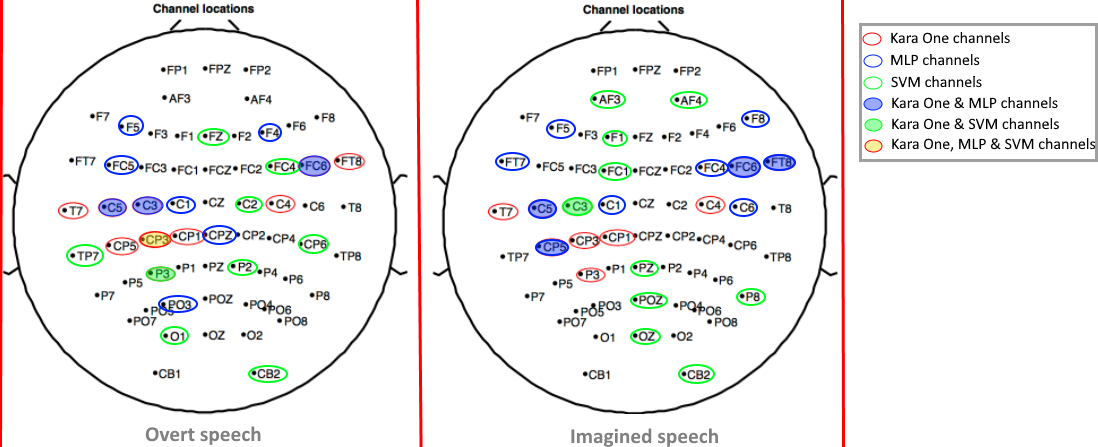
\includegraphics[width=\linewidth]{Figures/Channel_Selection.png}
	\caption{Selected channels in \cite{zhao2015classifying,zhao2013combining}, and those selected in this work for overt and imagined speech using MLP and SVM (Original Figure taken from \cite{karaone} for its adaptation in this work).}
	\label{Fig: Channel_Selection}
\end{figure}

\begin{table}[h!]
	\centering
	\caption{Example of channel's selection based on the best (average) F1 scores.}
	\scalebox{0.65}{
		\begin{tabular}{|*{11}{c|}}
			\hline
			\textbf{Ranking} & \textbf{1}     & \textbf{2}     & \textbf{3}     & \textbf{4}     & \textbf{5}     & \textbf{6}     & \textbf{7}     & \textbf{8}     & \textbf{9}     & \textbf{10} \\\hline
			\multirow{5}{*}{\begin{sideways}\textbf{Scores}\end{sideways}} & \cellcolor[rgb]{ 1,  .753,  0} 81.7204 & \cellcolor[rgb]{ 1,  .902,  .6} 72.7026 & \cellcolor[rgb]{ 1,  .753,  0} 71.7073 & 71.5593 & 70.2795 & 69.5274 & 69.2439 & 68.8333 & 67.5215 & 67.1659 \\\cline{2-11}
			& \cellcolor[rgb]{ 1,  .902,  .6} 75.6084 & \cellcolor[rgb]{ 1,  .902,  .6} 73.8739 & \cellcolor[rgb]{ 1,  .753,  0} 73.1938 & \cellcolor[rgb]{ 1,  .902,  .6} 72.2644 & \cellcolor[rgb]{ 1,  .753,  0} 71.6779 & 71.6777 & 71.6774 & 69.482 & 69.1112 & 68.6422 \\\cline{2-11}
			& \cellcolor[rgb]{ 1,  .902,  .6} 73.7852 & \cellcolor[rgb]{ 1,  .902,  .6} 73.1618 & 70.4938 & 70.4938 & 70.013 & 69.1816 & 67.9257 & 66.5594 & 65.625 & 65.2672 \\\cline{2-11}
			& \cellcolor[rgb]{ 1,  .902,  .6} 79.4051 & \cellcolor[rgb]{ 1,  .902,  .6} 77.1167 & \cellcolor[rgb]{ 1,  .902,  .6} 74.3707 & 70.8944 & 69.8651 & 69.0848 & 68.0152 & 67.7833 & 67.3944 & 66.9954 \\\cline{2-11}
			& \cellcolor[rgb]{ 1,  .753,  0} 82.9932 & \cellcolor[rgb]{ 1,  .753,  0} 82.0485 & \cellcolor[rgb]{ 1,  .753,  0} 76.1885 & \cellcolor[rgb]{ 1,  .753,  0} 74.2852 & \cellcolor[rgb]{ 1,  .753,  0} 73.9607 & \cellcolor[rgb]{ 1,  .753,  0} 73.2558 & 72.2323 & 70.8371 & 70.5964 & 69.6508 \\\hline
			\multirow{5}{*}{\begin{sideways}\textbf{Channels}\end{sideways}} & \cellcolor[rgb]{ 1,  .753,  0} CP6 & \cellcolor[rgb]{ 1,  .902,  .6} FZ & \cellcolor[rgb]{ 1,  .753,  0} CB2 & PO4   & FC1   & PO7   & T8    & CZ    & CPZ   & F6 \\\cline{2-11}
			& \cellcolor[rgb]{ 1,  .902,  .6} TP7 & \cellcolor[rgb]{ 1,  .902,  .6} CP6 & \cellcolor[rgb]{ 1,  .753,  0} FC4 & \cellcolor[rgb]{ 1,  .902,  .6} FZ & \cellcolor[rgb]{ 1,  .753,  0} P2 & C2    & FC5   & F1    & FC6   & T8 \\\cline{2-11}
			& \cellcolor[rgb]{ 1,  .902,  .6} O1 & \cellcolor[rgb]{ 1,  .902,  .6} C2 & FC4   & OZ    & FCZ   & CP4   & P5    & P4    & PO7   & FT7 \\\cline{2-11}
			& \cellcolor[rgb]{ 1,  .902,  .6} CP6 & \cellcolor[rgb]{ 1,  .902,  .6} FZ & \cellcolor[rgb]{ 1,  .902,  .6} TP7 & CPZ   & C5    & FC2   & FC6   & F1    & FC4   & O1 \\\cline{2-11}
			& \cellcolor[rgb]{ 1,  .753,  0} FZ & \cellcolor[rgb]{ 1,  .753,  0} C2 & \cellcolor[rgb]{ 1,  .753,  0} TP7 & \cellcolor[rgb]{ 1,  .753,  0} CP3 & \cellcolor[rgb]{ 1,  .753,  0} O1 & \cellcolor[rgb]{ 1,  .753,  0} P3 & FC4   & FC6   & FC5   & F1 \\\hline
			\textbf{Selection} & \cellcolor{orange}\textbf{FZ}    & \cellcolor{orange}\textbf{C2}    & \cellcolor{orange}\textbf{CP6}   & \cellcolor{orange}\textbf{TP7}   & \cellcolor{orange}\textbf{CP3}   & \cellcolor{orange}\textbf{O1}    & \cellcolor{orange}\textbf{P3}    & \cellcolor{orange}\textbf{FC4}   & \cellcolor{orange}\textbf{CB2}   & \cellcolor{orange}\textbf{P2} \\\hline
		\end{tabular}%
	}
	\label{Table: Channel_Selection_Example}%
\end{table}%

Notice that in this process, some elements in matrix $S$ had high F1 scores; however, they were discarded because the associated channels had been previously appended to the selection list (i.e. such channels had been identified before with a higher F1 score). These cases are highlighted in both matrices with pale yellow color.\\

It is also important to mention that other criteria were proposed previously to perform the channel's selection. Nevertheless, as happened with the other decisions, after performing some experiments, the best scores in the third step were obtained with the criterion exposed in Algorithm \ref{Algorithm: Channels}. The generalities of these other proposed criteria are described as follows:
\begin{itemize}
	\item \underline{Average Scores}: This criterion consisted of computing the average scores from $S$ between repeated channels based on $C$ items. Then, the average values are sorted and stored in $\vec{c}$, following the rest of the process as in Algorithm \ref{Algorithm: Channels}.
	\item \underline{Weighted Scores}: This criterion was similar to Average Scores. However, instead of averaging the repeated channels, they were summed and divided by $u$.
	\item \underline{Accuracy with F1 Scores}: This criterion consisted of counting the occurrences of each channel from the accuracy and F1 score matrices $C$. Then, the occurrence's lists are sorted in descending order to form the selected channel's ranking by the following priorities: 1) It was in both matrices, 2) it occurred more times in the F1 matrix than in the accuracy matrix, 3) it occurred in just F1 matrix but more than one time.
\end{itemize}

Finally, as a third step for Vector-based classification, just the $n$ classifiers that received feature vectors from the selected channels were used. However, in this step, both training and test data were introduced to the new architecture composed of $n$ classifiers, which each output a recognized class label. Once these $n$ labels were obtained, the decision rule (also shown in Figure \ref{Fig: Classification_VB}) was based on the class label's count.\\

If 70\% (or more) of the classifiers predicted the correct class label associated with the input sample, then such class is stated as the overall recognition. Otherwise, another class was randomly stated. Indeed, as binary classification experiments were performed for this work, the sample is associated with the other binary class
if less than 70\% of the classifiers predicted the correct class label.\\

Once collected the overall recognitions from all the training and test samples, all the score types were performed (accuracy, recall, precision, F1). However, just the accuracy score was reported in the classification results for simplification. Also, for the particular case of the MLP, this third step was executed 20 times again, and the average accuracies $\pm$ the standard deviations are reported.\\

\subsection{Spatio-Temporal}
\subsubsection{Encoding}
As a first step for the NeuCube, input signals were required to be encoded in spike trains since the neurons of the SNN captured, with their biological neuron model, the temporal information from them, while the connections represent the spatial information. Therefore, the problem was to select an encoding method that ensured the preservation of relevant information from the EEG signals by compressing them in spike trains.\\

Due to this concern, in \cite{petro2019selection} were tested different temporal spike encoding methods with several signal types that model a wide variety of behaviors. The approach adopted in that work was to compare the encoders' performance by computing some metrics based on the error between the original and reconstructed (or decoded) signals. The reconstruction of the signal refers to the process of transforming the resulting spike trains to EEG signals.\\

Hence, the error metrics computed in \cite{petro2019selection} were the SNR, RMSE, and R-squared measure. Thus, based on the resulting metric values from several performed experiments, it was concluded in \cite{petro2019selection} that the SF encoding method outperformed the others used there, which were BSA, TBR, and MW.\\

Notice that carrying experiments across encoding methods and error metrics (i.e., similarly as \cite{petro2019selection}) to select an adequate encoder for overt and imagined speech samples was out of scope for this work. Nevertheless, two encoding methods were selected and mutually compared based on their classification performance: SF \cite{kasabov2016evolving} and BSA \cite{schrauwen2003bsa}.\\

Additionally, instead of testing with several signals, the focus in this work consisted of performing optimization steps in each encoding method to minimize the RMSE.\\

SF was used due to the results and conclusions provided in \cite{petro2019selection}. Hence, the optimization process consisted of performing a grid search of the additive threshold value that provided the least RMSE. An optimal threshold value was obtained from and applied to each EEG signal. Therefore, the threshold values used for the grid search were the range from the EEG signal amplitudes by a factor varying from 0.001 to 0.8 with a step size of 0.001.\\

On the other hand, BSA was selected because it had been successfully applied in EEG signals in other earlier works \cite{kasabov2014neucube,nuntalid2011eeg}. Moreover, in  \cite{petro2019selection} was not performed any optimization procedure, and consequently, it was not explored this encoder thoroughly. In this work, a DEA \cite{storn1997differential} with constraints was used to obtain, similarly as for SF grid search, the optimal encoding per EEG signal by minimizing the RMSE.\\

For BSA optimization, the weighting factor, the crossover probability, and the number of generations were set to 0.02, 0.7, and 100, respectively. Additionally, as this encoding is based on an FIR filter, the constraints for the DEA were the filter order, the bandpass (radians per sample), and the BSA threshold with values between $[3,50]$, $[0.1,1]$, and $[0.2*maxValue,2*maxValue]$ (where $maxValue$ is the maximal value of the normalized signal), respectively.\\

In Table \ref{Table: BSA_Overt} and \ref{Table: BSA_Imagined} are shown for overt and imagined speech, respectively, the optimal values, as well as the RMSE, obtained after applying the DEA for BSA encoding of the 12 EEG signals from the $FC6$ channel corresponding to the class $/iy/$ from the subject $S_{1}$. Also, the last row shows the mean of each parameter value $\pm$ their variance.\\

Notice that although these signals belong to the same particular case (same subject, class, and channel), the optimal parameter's set founded vary per signal. Therefore, these results confirm the importance (and consequently the computational cost) of customizing the encoding process per signal.\\

Finally, Figure \ref{Fig: Encoded_Signals} illustrates an example of encoding EEG signals with both methods: SF and BSA. The plots from the first column belong to an overt speech signal, while those from the second column belong to an imagined speech signal. Indeed, both signals represent the same case: subject $S_{1}$, class $/iy/$, channel $FC6$, trial 1.\\

\begin{table}[h!]
	\centering
	\caption{Optimal values obtained after applying the DEA for BSA encoding: Overt Speech.}
	\begin{tabular}{|*{5}{c|}}
		\hline
		\textbf{Samples} & \textbf{Order} & \textbf{Bandpass} & \textbf{Threshold} & \textbf{RMSE} \\\hline
		1 & 28.271 & 0.17199 & 1.5127 & 0.038272 \\\hline
		2 & 38.921 & 0.11952 & 1.8157 & 0.035735 \\\hline
		3 & 30.141 & 0.11233 & 1.666 & 0.045256 \\\hline
		4 & 36.762 & 0.10304 & 1.7186 & 0.023799 \\\hline
		5 & 30.952 & 0.14482 & 1.65 & 0.043209 \\\hline
		6 & 38.093 & 0.18224 & 1.5182 & 0.059114 \\\hline
		7 & 31.103 & 0.25417 & 1.0692 & 0.097987 \\\hline
		8 & 14.593 & 0.18057 & 1.6381 & 0.058363 \\\hline
		9 & 19.213 & 0.15574 & 1.5316 & 0.052366 \\\hline
		10 & 26.39 & 0.13468 & 1.7515 & 0.018461 \\\hline
		11 & 25.488 & 0.12689 & 1.4348 & 0.051495 \\\hline
		12 & 21.431 & 0.11995 & 1.88 & 0.046047 \\\hline
		\textbf{Mean}  & \textbf{28.45$\pm$7.55} & \textbf{0.151$\pm$0.04} & \textbf{1.5989$\pm$0.21} & \textbf{0.0475$\pm$0.02} \\\hline
	\end{tabular}%
	\label{Table: BSA_Overt}%
\end{table}%

\begin{table}[h!]
	\centering
	\caption{Optimal values obtained after applying the DEA for BSA encoding: Imagined Speech.}
	\begin{tabular}{|*{5}{c|}}
		\hline
		\textbf{Samples} & \textbf{Order} & \textbf{Bandpass} & \textbf{Threshold} & \textbf{RMSE} \\\hline
		1 & 28.85 & 0.22533 & 1.2691 & 0.092413 \\\hline
		2 & 30.896 & 0.13097 & 1.4116 & 0.13636 \\\hline
		3 & 45.052 & 0.19549 & 1.3476 & 0.15121 \\\hline
		4 & 48.274 & 0.20386 & 1.1463 & 0.14691 \\\hline
		5 & 31.041 & 0.22677 & 1.0035 & 0.15148 \\\hline
		6 & 10.811 & 0.1405 & 1.2954 & 0.16745 \\\hline
		7 & 12.54 & 0.29571 & 1.3338 & 0.091356 \\\hline
		8 & 13.618 & 0.17725 & 1.4635 & 0.12126 \\\hline
		9 & 20.785 & 0.25031 & 1.3084 & 0.1089 \\\hline
		10 & 31.744 & 0.16863 & 1.3277 & 0.11905 \\\hline
		11 & 8.1956 & 0.28021 & 1.3053 & 0.11948 \\\hline
		12 & 14.674 & 0.13437 & 1.4901 & 0.11043 \\\hline
		\textbf{Mean}  & \textbf{24.71$\pm$13.4} &\textbf{ 0.203$\pm$0.06} & \textbf{1.3085$\pm$0.13} & \textbf{0.1264$\pm$0.02} \\\hline
	    \end{tabular}%
	\label{Table: BSA_Imagined}%
\end{table}%

\begin{figure}[h!]
\centering
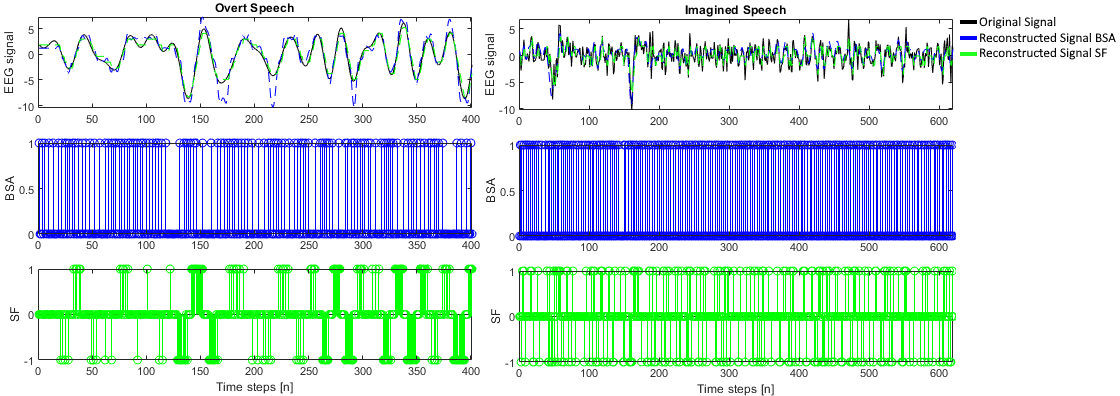
\includegraphics[width=\linewidth]{Figures/Encoded_Signals.png}
\caption{Encoded signal examples using SF and BSA.}
\label{Fig: Encoded_Signals}
\end{figure}

Thus, in both columns, the first plot shows the original EEG signal in black, as well as the reconstructed signal after applying the BSA and SF encoding in dashed blue and green lines, respectively. Notice that for these examples, SF reconstructed the overt speech signal better than BSA, while for the imagined speech signal was the opposite case.\\

Besides, the second pair of plots show the spike trains after applying BSA, which provides just positive spikes. Whereas, the third pair of plots correspond to the encoded signal after applying SF, which provides positive and negative spikes.\\

\subsubsection{Classification}
After all the samples were encoded, the following methodology was performed to select the data for a grid search that would allow optimizing the parameters of the NeuCube for the classification step:\\
\begin{enumerate}
	\item Overt and imagined speech data were selected from the binary classes ($\pm$Nasal or $\pm$Bilabial),  and the codification applied (BSA or SF). The combination of such cases resulted in 4 data sets per mental task (overt or imagined speech).
	\item Then, for each data set, just the samples of $S_{1}$ were taken as test data since that subject produced more trials. Experiments by taking the samples of the other subjects as test data were not performed in this step due to the long-time they would consume following this methodology.
	\item Next, several classification experiments were performed by varying the percent of excitatory connections ($r_{+}$) and LIF threshold ($\vartheta$) once the training and test data were stated per data set. Therefore, the overall accuracy (sum of training and test accuracies divided by two) was registered per case, and the same initialization was used across all the cases (i.e., just one experiment was performed per case).
	\item Later, the parameter pairs (8 in total) that provided the best overall accuracy per mental task and data set were selected for the next step in this methodology. Table \ref{Table: NeuCube_Dataset_Params} shows the overall accuracies across all the cases, and the best, and consequently selected, are highlighted.
	\item As the last step, these best parameter pairs were used again (with their corresponding mental task and data set samples) but now following the validation methodology described in the next chapter, which provides accuracies that represent when each subject's data were used for testing. This step was done to select the subject's test data for the grid search. Table \ref{Table: NeuCube_TestSelection} shows the resulting overall accuracies from 10 different initializations. Besides, the best results for overt and imagined speech samples are highlighted, which were also the data set samples used for the grid search of such mental tasks.
\end{enumerate}

\begin{table}[h!]
	\centering
	\caption{Overall accuracies for NeuCube data set parameter's selection.}
	\begin{tabular}{|*{7}{c|}}
		\cline{4-7}
		\multicolumn{3}{c|}{\multirow{1}{*}{}} & \multicolumn{2}{c|}{\textbf{Overt Speech}} & \multicolumn{2}{c|}{\textbf{Imagined Speech}} \\\cline{2-7}
		\multicolumn{1}{c|}{\multirow{1}{*}{}}  & \boldmath$r_{+}$ & \boldmath$\vartheta$ & \textbf{BSA} & \textbf{SF} & \textbf{BSA} & \textbf{SF} \\\hline
		\multirow{4}{*}{\begin{sideways}\textbf{Nasal}\end{sideways}} & \cellcolor{orange}0.7   & \cellcolor{orange}0.1   & 58.35 & 59.14 & 57.87 & \cellcolor{orange}60.19 \\\cline{2-7}
		& 0.7   & 0.05  & 58.61 & 58.97 & 47.22 & 55.46 \\\cline{2-7}
		& \cellcolor{orange}0.5   & \cellcolor{orange}0.1   & \cellcolor{orange}59.62 & \cellcolor{orange}61.64 & \cellcolor{orange}59.53 & 54.89 \\\cline{2-7}
		& 0.5   & 0.05  & 53.53 & 55.42 & 48.01 & 54.62 \\\hline
		\multirow{4}{*}{\begin{sideways}\textbf{Bilabial}\end{sideways}} & \cellcolor{orange}0.7   & \cellcolor{orange}0.1   & 59.67 & 58.26 & 50.37 & \cellcolor{orange}59.01 \\\cline{2-7}
		& 0.7   & 0.05  & 53.00 & 57.69 & 46.03 & 54.23 \\\cline{2-7}
		& \cellcolor{orange}0.5   & \cellcolor{orange}0.1   & \cellcolor{orange}62.08 & \cellcolor{orange}60.02 & \cellcolor{orange}52.21 & 58.18 \\\cline{2-7}
		& 0.5   & 0.05  & 58.48 & 58.83 & 49.59 & 55.33 \\\hline
	\end{tabular}%
	\label{Table: NeuCube_Dataset_Params}%
\end{table}%

\begin{table}[h!]
	\centering
	\caption{Overall accuracies for NeuCube samples selection for grid search.}
	\begin{tabular}{|*{6}{c|}}
		\cline{3-6}
		\multicolumn{2}{c|}{\multirow{1}{*}{}} & \multicolumn{2}{c|}{\textbf{Overt Speech}} & \multicolumn{2}{c|}{\textbf{Imagined Speech}} \\\cline{2-6}
		\multicolumn{1}{c|}{\multirow{1}{*}{}}  & \textbf{Subject} & \textbf{BSA} & \textbf{SF} & \textbf{BSA} & \textbf{SF} \\\hline
		\multirow{5}{*}{\begin{sideways}\textbf{Nasal}\end{sideways}} & $S_{1}$    & 59.68 & 55.86 & 56.25 & 54.87 \\\cline{2-6}
		& $S_{2}$    & 58.23 & 56.44 & 54.53 & 54.95 \\\cline{2-6}
		& $S_{3}$    & 55.69 & 57.55 & 54.62 & 55.22 \\\cline{2-6}
		& $S_{4}$    & 58.71 & 58.22 & 54.61 & 55.08 \\\cline{2-6}
		& \cellcolor{orange}$S_{5}$    & 59.68 & \cellcolor{orange}60.74 & 51.34 & 55.55 \\\hline
		\multirow{5}{*}{\begin{sideways}\textbf{Bilabial}\end{sideways}} & $S_{1}$    & 56.93 & 58.24 & 52.18 & 57.96 \\\cline{2-6}
		& $S_{2}$    & 58.66 & 56.01 & 54.46 & 56.10 \\\cline{2-6}
		& $S_{3}$    & 53.01 & 57.52 & 55.51 & 57.17 \\\cline{2-6}
		& \cellcolor{orange}$S_{4}$    & 58.66 & 56.75 & 53.83 & \cellcolor{orange}58.31 \\\cline{2-6}
		& $S_{5}$    & 57.27 & 57.62 & 54.71 & 54.94 \\\hline
	\end{tabular}%
	\label{Table: NeuCube_TestSelection}%
\end{table}%

\begin{table}[h!]
\caption{Grid search values used for the NeuCube.}
\centering
\begin{tabular}{|c|c|}\hline
	\textbf{Parameters}&\textbf{Values}\\\hline
	$r_{+}$&{0.3, 0.5, 0.7}\\\hline
	$\vartheta$&{0.05, 0.07, 0.08, 0.1, 0.11, 0.13}\\\hline
	$\pm A$&{0.001, 0.005, 0.01}\\\hline
	$\pm D$&{0.001, 0.005, 0.01}\\\hline
\end{tabular}
\label{Table: NeuCube_Gridsearch}
\end{table}

Finally, based on the selected data sets ($\pm$Nasal, SF, $S_{5}$ test data for overt speech; $\pm$Bilabial, SF, $S_{4}$ test data for imagined speech), Table \ref{Table: NeuCube_Gridsearch} shows the values used for some NeuCube parameters in a grid search per mental task. Performing the grid search for all the NeuCube parameters was not realizable due to time-consuming.\\

After these grid searches, the parameter set founded was stated for the definitive \linebreak[4]classification of all samples. This definitive classification consisted of computing the training and test scores with the validation methodology using 20 different NeuCube initializations but with the same parameter set.

\subsection{Mixed Approach}
The SSN performs the classification step in a Spatio-temporal approach by multiplying all EEG channel data at once with their corresponding input weights per time step. However, it is considered as a mixed approach classifier in this work since it was fed with EEG preprocessed signals (following the corresponding Spatio-temporal steps) as well as with feature vectors (which implied processing and feature extraction steps of the Vector-based approach). Despite the differences between step approaches, the experiments were performed with the same conditions for both input data types.\\

Contrary to the NeuCube experiments, for the SNN were used two different neuron models: LIF and Izhikevich. This last was not used in the NeuCube because the variables model's combinations can represent 27 different behaviors of the neuron, which was not viable to test each of them per case. However, it was possible to apply Izhikevich model for the SSN due to the DEA of \cite{storn1997differential} employed during the training step. Additionally, performing the DAE over Izhvikevich model had the advantage of using just the behaviors that prevailed on every new generation instead of testing all of them.\\

Furthermore, by using the DEA, each individual was a vector composed of the 62 input weight values on the interval $[-0.01,0.01]$ and the neuron model parameters to tune. In the case of the LIF model, these parameters were the refractory period and the threshold ($\vartheta$) values on the intervals $[0,6] \in \mathbb{Z}$ and $[0.1,1]$, respectively. On the other hand, the only parameter used for the Izhikevich model was the behavior's identifier, from which its interval values were $[0,27] \in \mathbb{Z}$. Additionally, the population size per generation was set to 10 times the length of the individuals; i.e., the number of individuals for the LIF and the Izhikevich model was 640 and 630, respectively.\\

Notice that the SSN training step (explained in Chapter 3 of this thesis) implied an internal optimization process, which consisted of minimizing the error by selecting the best individuals for the next generation in the DEA. Consequently, the SSN did not require any other score improvement as in the Vector-based approach (with a channel's selection step) or the NeuCube (with a grid search).\\

Figure \ref{Fig: SSN_Error} shows the number of errors obtained per generation for both mental tasks (overt and imagined speech) during the training step, from which the LIF neuron model, $\pm$Bilabial sets, and $S_{3}$ test data were used. However, in these examples, 21-feature vectors were used as input for overt speech; while, EEG signals were used for imagined speech.\\

Hence, the blue and red curves represent, respectively, the best and the worst-case per generation. Besides, the green curve represents the average number of errors across all the individuals per generation, and the yellow lines are the $\pm$standard deviation from the average error, which had few variations across the generations.\\

Notice that for both cases in the examples of Figure \ref{Fig: SSN_Error}, after 200 generations, the blue curve started to decreased less. In the end, the SSN configured with the best individual (from the 500th generation) misclassified 137 and 157 samples for overt and imagined speech, respectively, during the training step.\\

\begin{figure}[h!]
	\centering
	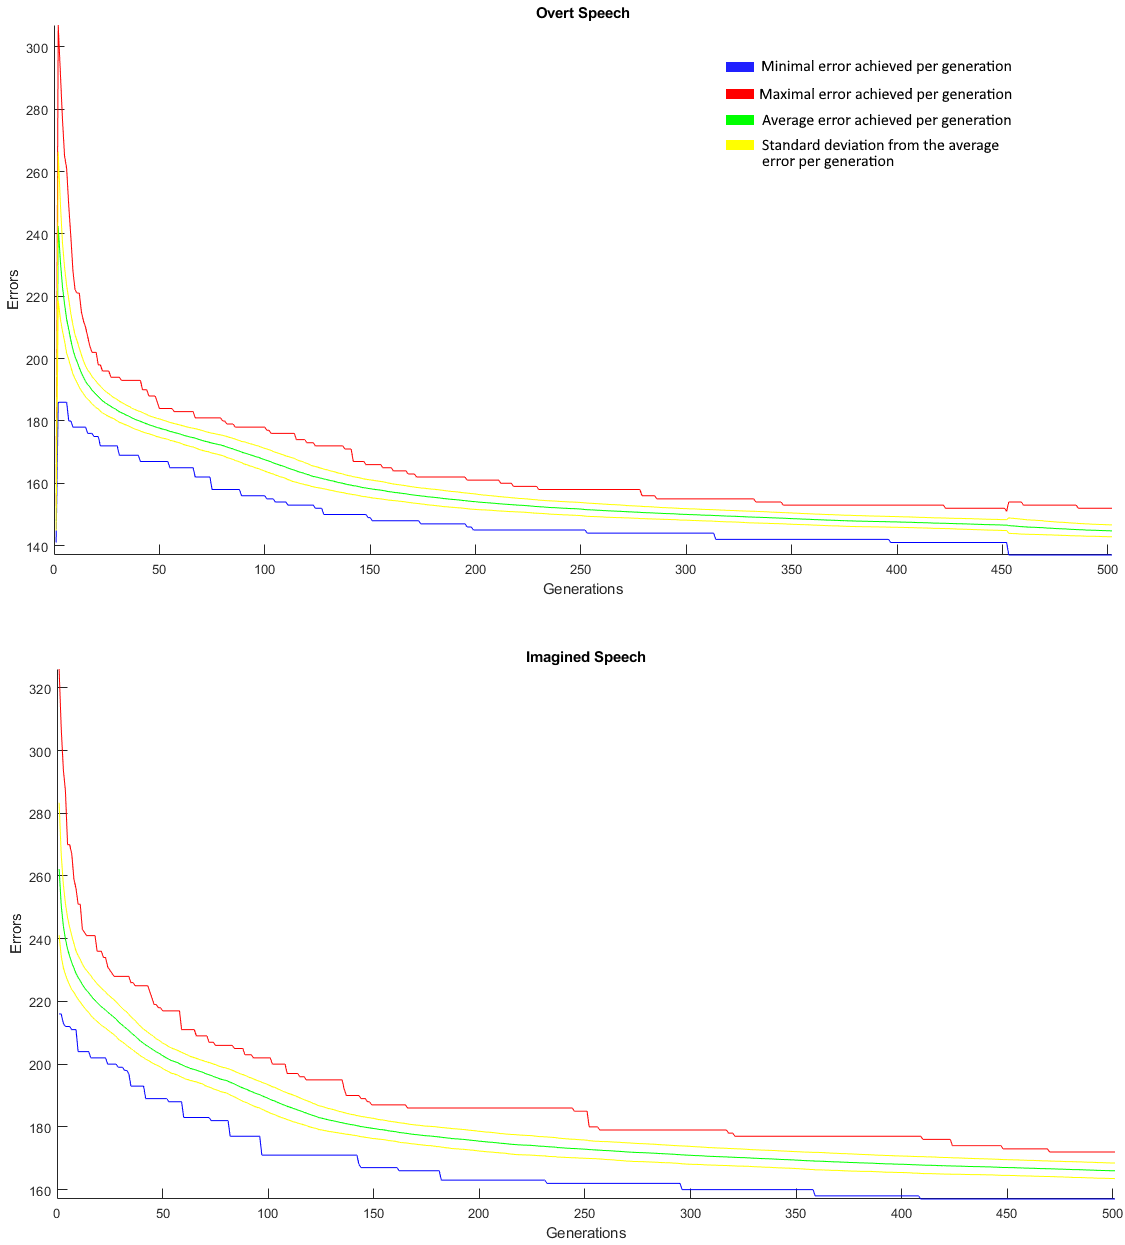
\includegraphics[width=\linewidth]{Figures/SSN_Error.png}
	\caption{Number of errors per generation during SSN training for overt and imagined speech examples.}
	\label{Fig: SSN_Error}
\end{figure}

These last and best SSN configurations were used for the test step, which consisted of passing the test samples through the SSN. Then, their firing rates were computed and compared with the AFRs from both classes to associate them with the closest. Finally, the scores were computed based on the errors produced in the classification.\\